\documentclass[10pt,a4paper]{article}
\usepackage{amsmath,amssymb,amsthm,graphicx}
\usepackage{amsfonts,amssymb,amsmath,amsthm,mathtools,graphicx,bm,xspace,booktabs,array,multirow,dsfont}
\usepackage{enumitem}
\setlist[itemize]{noitemsep}
\setlist[enumerate]{noitemsep}
\usepackage[usenames,dvipsnames]{xcolor}
\definecolor{Gred}{RGB}{219,50,54}
\definecolor{Ggreen}{RGB}{60,186,84}
\definecolor{Gblue}{RGB}{72,133,237}
\definecolor{Gyellow}{RGB}{247,178,16}
\definecolor{ToCgreen}{RGB}{0,128,0}
\definecolor{myGold}{RGB}{231,141,20}
\definecolor{myBlue}{rgb}{0.19,0.41,.65}
\definecolor{myPurple}{RGB}{175,0,124}
\usepackage[colorlinks=true,hypertexnames=false]{hyperref}
\usepackage{tikz}
\usetikzlibrary{arrows.meta,shapes}
\usepackage[framemethod=tikz]{mdframed}
\mdfsetup{roundcorner=4pt,linewidth=.5,innerleftmargin=10pt,innerrightmargin=10pt,innertopmargin=10pt,innerbottommargin=10pt}
\usepackage{thmtools,thm-restate}
\usepackage[no-math]{fontspec}
\newtheorem{theorem}{Theorem}
\newtheorem{lemma}[theorem]{Lemma}
\newtheorem{corollary}[theorem]{Corollary}
\newtheorem{proposition}[theorem]{Proposition}
\newtheorem{claim}[theorem]{Claim}
\newtheorem{fact}[theorem]{Fact}
\newtheorem{techlemma}[theorem]{Technical Lemma}
\theoremstyle{definition}
\newtheorem{definition}[theorem]{Definition}
\theoremstyle{remark}
\newtheorem{remark}[theorem]{Remark}
\newtheorem{example}[theorem]{Example}
\newenvironment{Enumerate}{\begin{enumerate}}{\end{enumerate}}
\newenvironment{Itemize}{\begin{itemize}}{\end{itemize}}
\newcommand{\contour}[2]{#2}
\let\boldm\bm
\newenvironment{nproblem}[1][\unskip]{\medskip\begin{mdframed}\noindent\underline{$#1$ Problem.}\\\noindent}{\end{mdframed}}
\allowdisplaybreaks
\AtBeginDocument{\author{\parbox{.95\textwidth}{\centering Mika G\"o\"os, Pritish Kamath,\\ Katerina Sotiraki, Manolis Zampetakis}}}

\newcommand{\inparen}[1]{\left ( #1 \right )}
\newcommand{\infork}[1]{\left \{ \begin{matrix} #1 \end{matrix} \right .}
\newcommand{\inabs}[1]{\begin{vmatrix} #1 \end{vmatrix}}
\renewcommand{\mod}[1]{~\inparen{\mathrm{mod}~#1}}
\newcommand{\bx}{{\boldm x}}
\def\ceil#1{\mathop{\left\lceil#1\right\rceil}}
\def\abs#1{\left|#1\right|}
\def\p#1{\left(#1\right)}
\def\a#1{\langle#1\rangle}
\def\set#1{\left\{#1\right\}}
\newcommand{\parasc}[1]{\noindent \contour{black}{#1}}
\newcommand{\paragr}[1]{\noindent \textbf{\boldmath #1}}
\newcommand{\F}{\ensuremath{\mathbb{F}}}
\newcommand{\bbF}{\ensuremath{\mathbb{F}}}
\newcommand{\bbZ}{\ensuremath{\mathbb{Z}}}
\newcommand{\calC}{\mathcal{C}}
\newcommand{\calG}{\mathcal{G}}
\newcommand{\calM}{\mathcal{M}}
\newcommand{\calR}{\mathcal{R}}
\newcommand{\calT}{\mathcal{T}}
\newcommand{\calV}{\mathcal{V}}
\renewcommand{\vec}[1]{\boldsymbol{#1}}
\newcommand{\vecf}{\ensuremath{\boldsymbol{f}}}
\newcommand{\vecg}{\ensuremath{\boldsymbol{g}}}
\newcommand{\vech}{\ensuremath{\boldsymbol{h}}}
\newcommand{\vecv}{\ensuremath{\boldsymbol{v}}}
\newcommand{\vecx}{\ensuremath{\boldsymbol{x}}}
\newcommand{\vecy}{\ensuremath{\boldsymbol{y}}}
\newcommand{\vecz}{\ensuremath{\boldsymbol{z}}}
\newcommand{\bit}{\ensuremath{\set{0,1}}}
\DeclareMathOperator*{\poly}{\ensuremath\mathrm{poly}}
\newcommand{\problem}[1]{\ensuremath{\textsc{#1}}\xspace}
\newcommand{\class}[1]{\ensuremath{\mathsf{#1}}\xspace}
\newcommand{\FNP}{\class{FNP}}
\newcommand{\TFNP}{\class{TFNP}}
\newcommand{\PPA}{\class{PPA}}
\newcommand{\PPAp}{\class{PPA}_{{p}}}
\newcommand{\sis}{\problem{SIS}}
\newcommand{\pnum}{p}
\newcommand{\qnum}{q}
\newcommand{\lonelyp}{\ensuremath\textsc{Lonely}_{\pnum}}
\newcommand{\bipartitep}{\ensuremath{\textsc{Bipartite}_{\pnum}}}
\newcommand{\twoMatchingsp}{\ensuremath{\textsc{TwoMatchings}_{\pnum}}}
\newcommand{\sucBipartitep}{\ensuremath{\textsc{SuccinctBipartite}_{\pnum}}}
\newcommand{\leafq}{\ensuremath\textsc{Leaf}_{\qnum}}
\newcommand{\lonelyq}{\ensuremath\textsc{Lonely}_{\qnum}}
\newcommand{\bipartiteq}{\ensuremath{\textsc{Bipartite}_\qnum}}
\newcommand{\leaf}{\ensuremath\textsc{Leaf}}
\newcommand{\lonely}{\ensuremath\textsc{Lonely}}
\newcommand{\bipartite}{\ensuremath{\textsc{Bipartite}}}
\newcommand{\twoMatchings}{\ensuremath{\textsc{TwoMatchings}}}
\newcommand{\sucBipartite}{\ensuremath{\textsc{SuccinctBipartite}}}
\newcommand{\reducible}{\preceq}
\newcommand{\Chevalley}{\ensuremath\textsc{Chevalley}}
\newcommand{\CWT}{CWT\xspace}
\newcommand{\lChevalleyp}{\textsc{GeneralChevalley}_{\pnum}}
\newcommand{\cChevalleyp}{\textsc{ChevalleyWithSymmetry}_{\pnum}}
\newcommand{\eChevalleyp}{\textsc{Chevalley}_{\pnum}}
\newcommand{\lChevalley}{\textsc{GeneralChevalley}}
\newcommand{\cChevalley}{\textsc{ChevalleyWithSymmetry}}
\newcommand{\eChevalley}{\textsc{Chevalley}}
\newcommand{\CW}{\mathsf{CW}}

\providecommand{\bigtimes}{\mathop{\times}\displaylimits}
\providecommand{\bracks}[1]{\left[#1\right]}
\title{Explicit Chevalley-Warning-with-symmetry search is PPA\_p-complete for prime p}
\author{Mika Göös, Pritish Kamath, Katerina Sotiraki, Manolis Zampetakis}
\date{doi:10.4230/LIPIcs.CCC.2020.19; CC BY 3.0 Unported}
\begin{document}
\maketitle
\noindent\textit{Editorial scope.} One explicit ChevalleyWithSymmetry\_p completeness mechanism with full membership/hardness,monomial/symmetry/labeled-CWT and required graph equivalence proofs. Only prime p. Ordinary Chevalley\_p completeness remains unclaimed;SIS background is not upgraded or counted. Independent q classification not counted in this task.\par\medskip
\noindent\textit{Allowed standard prerequisites (editorial).}\begin{itemize}
\item Finite-field polynomial arithmetic,modulo-p counting,free cyclic actions and TFNP many-one reductions. Actual p is prime,q denotes an integer>=2. Standard finite-field/counting facts remain background;all author CWT/monomial/symmetry/labeled-degree and local graph/reduction proofs are retained. Full37 formal bibliography entries retained.
\end{itemize}\medskip
\setcounter{section}{1}
\setcounter{subsection}{1}
\setcounter{theorem}{1}
\subsection{A Natural Complete Problem via Chevalley-Warning Theorem}
\label{sec:intro-complete}

There have been several works focusing on completeness results for the class $\PPA$ (i.e. $\PPA_2$). Initial works showed the
$\PPA$-completeness of (non-natural) total search problems corresponding to topological fixed point theorems
\cite{r24,r1,r19}. Closer to our paper,
Belovs et al. \cite{r8} show the $\PPA$-completeness of computational analogs of Combinatorial Nullstellensatz and the Chevalley--Warning Theorem, but which explicitly
involve a circuit as part of the input. More recently, breakthrough results
showed $\PPA$-completeness of problems without a circuit or a Turing Machine in
the input such as $\textsc{Consensus-Halving}$, $\textsc{Necklace-Splitting}$
and $\textsc{Ham-Sandwich}$
\cite{r20,r21} resolving an open
problem since the definition of $\PPA$ in \cite{r33}.

  Our main contribution is to provide a natural complete problem for $\PPA_p$,
for every prime $p$; thereby also yielding a new complete problem for $\PPA$.
Our complete problem is an extension of the problem $\eChevalleyp$, defined by
Papadimitriou \cite{r33}, which is a search problem
associated to the celebrated Chevalley-Warning Theorem. We first
present an abstract way to understand the proof of the Chevalley-Warning Theorem
that motivates the definition of our natural complete problem for
$\PPA_p$.

\subsubsection{Max-Degree Monic Monomials and Proof of Chevalley-Warning Theorem} \label{sec:maximum-degree}

  In 1935, Claude Chevalley \cite{r15} resolved a
hypothesis stated by Emil Artin, that all finite fields are quasi-algebraically
closed. Later, Ewald Warning~\cite{r37}
proved a slight generalization of Chevalley's theorem. This
generalized statement is usually referred to as the Chevalley-Warning Theorem
(\CWT, for short). Despite its initial algebraic motivation, \CWT has found
profound applications in combinatorics and number theory as we discuss in
Section1.4 (and Section6).

We now explain the statement of the Chevalley-Warning Theorem, starting with some notations. For any field $\bbF$ and any polynomial $f$ in a polynomial ring $\bbF[x_1, \ldots, x_n]$ we use $\deg(f)$ to represent the degree of $f$. We use $\vecx$ to succinctly denote the set of all variables $(x_1, \ldots, x_n)$ (the number of variables will always be $n$) and $\vecf$ to succinctly denote a system of polynomials $\vecf = (f_1, \ldots, f_m) \in \bbF[\vecx]^m$. We will often abuse notations to use $\bx$ to also denote assignments over $\bbF_p^n$. For instance, let $\calV_{\vecf} \coloneqq \set{\bx \in \bbF_p^n : f_i(\bx) = 0 \text{ for all } i \in [m]}$ be the set of all common roots of $\vecf$.

\theoremstyle{plain}
\newtheorem*{cwthm}{Chevalley-Warning Theorem}
\begin{cwthm}[\cite{r15,r37}]
For any prime\footnote{While most of the results in this section
generalize to prime powers, we only consider prime fields for simplicity.} $p$ and polynomial system
$\vecf \in \bbF_p[\vecx]^m$ satisfying\vspace{-3.5mm}
\begin{equation}
\tag{CW Condition}
\sum_{i = 1}^m \deg(f_i) < n,\vspace*{-3mm}
\label{eq:CWcondition}
\end{equation}
it holds that $|\calV_{\vecf}| \equiv 0 \mod{p}$.
\end{cwthm}

\noindent Given a polynomial system $\vecf \in \bbF_p[\vecx]^m$,
the key idea in the proof of the Chevalley-Warning Theorem is the polynomial
\[ \CW_{\vecf}(\bx) \coloneqq \prod_{i = 1}^m \inparen{1 - f_i(\vecx)^{p - 1}} \mod{\set{x_i^p - x_i}_i}\,. \] Observe that $\CW_{\vecf}(\vecx) = 1$ if $\vecx \in \calV_{\vecf}$ and is $0$ otherwise. Thus, $|\calV_{\vecf}| \equiv \sum_{\vecx \in \bbF_p^n} \CW_{\vecf}(\bx) \mod{p}$.
The following definition informally describes a special type of monomial of
$\CW_{\vecf}$ that is of particular interest in the proof. For the precise definition, we
refer to \autoref{sec:chevalley}.

\begin{definition}[\textsc{Max-Degree Monic Monomials} (Informal)]
	\label{def:max-degreeMonomialInformal}
    Let $\vecf \in \bbF_p[\vecx]^m$.
    			A \textit{monic monomial} of $\CW_{\vecf}$ refers to a monic monomial obtained when symbolically expanding $\CW_{\vecf}$ as a sum of monic monomials. A monic monomial is said to be of \textit{max-degree} if it is
	$\prod_{j = 1}^n x_j^{p - 1}$.

\end{definition}

   In the above definition, it is important to consider the
\emph{symbolic expansion} of $\CW_{\vecf}$ and ignore any cancellation of coefficients that might occur. Observe that, although the
expansion of $\CW_{\vecf}$ is exponentially large in the description size of
$\vecf$, each monic monomial of $\CW_{\vecf}$ can be succinctly described as a combination of monic monomials of the polynomials $f_1, \ldots, f_m$. We formally
discuss this in \autoref{sec:chevalley}.

Using the definition of max-degree monic monomials, we state the main technical
lemma underlying the proof of \CWT (with proof in \autoref{sec:chevalley}).
\theoremstyle{plain}
\newtheorem*{cwthmprinciple}{Chevalley--Warning Lemma}
\begin{cwthmprinciple}
For any prime $p$ and $\vecf \in \bbF_p[\vecx]^m$,
\begin{equation}
	\tag{CW Lemma}
	|\calV_{\vecf}| ~\equiv~ (-1)^n \cdot  |\set{\mathrm{max\text{-}degree~monic~monomials~of~} \CW_{\vecf}}| \mod{p}
	\label{eq:mainPrinciple}
\end{equation}
\end{cwthmprinciple}

\noindent The Chevalley-Warning Theorem now follows by observing that if $\sum_{i = 1}^m \deg(f_i) < n$ then the number of max-degree monic monomials of $\CW_{\vecf}$ is zero. Hence, we get that $|\calV_{\vecf}| \equiv 0 \mod{p}$.

\subsubsection{Proofs of Cancellation}
\label{sec:proofsOfCancellation}

  From the proof sketch of CWT in the previous section, a slight generalization of CWT follows. In particular, $|\calV_{\vecf}| \equiv 0 \mod{p}$ if and only if
\begin{equation}
	\tag{Extended CW Condition}
	\inabs{\set{\mathrm{max\text{-}degree~monic~monomials~of~} \CW_{\vecf}}} ~\equiv~ 0 \mod{p},
		\label{eq:generalizedCondition}
\end{equation}
Thus, any condition on $\vecf$ that implies the \eqref{eq:generalizedCondition} can
 replace \eqref{eq:CWcondition} in the Chevalley-Warning
Theorem. Note that the \eqref{eq:generalizedCondition} is equivalent to all the max-degree monic monomials in $\CW_{\vecf}$ cancelling out.
Thus, we call any such condition on $\vecf$ that implies \eqref{eq:generalizedCondition} to be a
``\textit{proof of cancellation}'' for the system $\vecf$.

We can now reinterpret the result of Belovs et
al. \cite{r8} in this framework of ``proof of cancellation'' conditions. In particular, \cite{r8} considers the
case $p = 2$ and defines the problem $\textsc{PPA-Circuit-Chevalley}$, in which a ``proof of
cancellation'' is given in a specific form of circuits. These circuits describe the
system $(f_1, \ldots, f_m)$ in the $\textsc{PPA-Circuit-Chevalley}$ problem. It is then shown that $\textsc{PPA-Circuit-Chevalley}$ is $\PPA_2$-complete.


\subsubsection{Computational Problems Based on Chevalley-Warning Theorem}
\label{sec:computationalChevalleyWarning}

  Every ``proof of cancellation'' that is \textit{syntactically refutable} can be used to define
  a total search problem that lies in $\PPA_p$. By {\em syntactically refutable} we mean that whenever the
  ``proof of cancellation'' is false, there exists a small witness that certifies so. In this
  section, we define three computational problems with their corresponding ``proof of
  cancellation'': (1) the $\eChevalleyp$ problem defined by \cite{r33}, (2) the
  $\lChevalleyp$ problem that is a generalization of $\eChevalleyp$, and (3) the problem
  $\cChevalleyp$ that we show to be $\PPA_p$-complete. All these problems are
  defined for every prime modulus $p$ and are natural in the sense that they do not explicitly
  involve a circuit or a Turing Machine in their input. In particular, the polynomial systems in the input are {\em explicit} in that they are given as a sum of monic monomials. \bigskip

\paragraph{Chevalley.}
  This is the direct computational analog of the Chevalley-Warning Theorem and was
defined by Papadimitriou \cite{r33} as the following total
search problem:
\medskip

\noindent $\underbar{\eChevalley}_{\pnum}$

\noindent Given an explicit polynomial system $\vecf \in \bbF_p[\vecx]^m$, and an
$\vecx^{\star} \in \calV_{\vecf}$, output one of the following:\vspace*{-0.8mm}
\begin{itemize}
	\item[$\triangleright$] [{\em Refuting witness}] \eqref{eq:CWcondition} is not satisfied.
	\item[$\triangleright$] $\vecx \in \calV_{\vecf} \smallsetminus \set{\vecx^{\star}}$.
\end{itemize}

\noindent We will particularly consider a special case where all the $f_i$'s have zero constant term
({\em zecote}, for short). In this case, $\vecx^{\star} = \mathbf{0} \in \calV_{\vecf}$, so there is no need to explicitly include $\vecx^*$ in the input.

\paragraph{General Chevalley.} As mentioned already, we can define a search problem corresponding to any syntactically refutable condition that implies the
\eqref{eq:generalizedCondition}. One such condition is to directly assert that\vspace{-2.5mm}
\begin{equation}
	\tag{General CW Condition}
	\{\mathrm{max\text{-}degree~monic~monomials~of~} \CW_{\vecf}\} ~=~ \emptyset. \label{eq:generalCWCondition}
\end{equation}
In particular, note that \eqref{eq:CWcondition} implies this condition. Moreover, this condition is syntactically refutable by a max-degree monic monomial, which is efficiently representable as a combination of at most $m(p-1)$ monomials of the $f_i$'s. Thus, we can define the following total search problem generalizing $\eChevalleyp$.\medskip

\noindent $\underbar{\lChevalley}_{\pnum}$

\noindent Given an explicit polynomial system $\vecf \in \bbF_p[\vecx]^m$ and an
$\vecx^{\star} \in \calV_{\vecf}$, output one of the following:\vspace{-0.5mm}
\begin{itemize}
	\item[$\triangleright$] [{\em Refuting Witness}] A max-degree monic monomial of $\CW_{\vecf}$.
	\item[$\triangleright$] $\vecx \in \calV_{\vecf} \smallsetminus \set{\vecx^{\star}}$.
\end{itemize}
\medskip

\noindent While $\lChevalleyp$ generalizes $\eChevalleyp$, it does not
capture the full generality of \eqref{eq:generalizedCondition}. However \eqref{eq:generalizedCondition} is not syntactically refutable (in fact, it is $\mathsf{Mod}_p\mathsf{P}$--complete to decide\footnote{Circuit-SAT can be encoded as satisfiability of a polynomial system $\vecf \in \bbF_p[\vecx]^m$ by including a polynomial for each gate along with $\set{x_i^2 - x_i = 0}$ to ensure Booleanity. Thus, number of satisfiable assignments to the Circuit-SAT is $\equiv |\calV_{\vecf}| \mod{p}$, which is $0 \mod{p}$ iff the final coefficient of the max-degree monomial is $0$.} if the final coefficient of the max-degree monomial is $0$).

A natural question then is whether $\lChevalley_p$, or even $\Chevalley_p$, could already be $\PPA_p$--complete. We believe this to be unlikely because \eqref{eq:generalCWCondition} seems to fail in capturing other simple conditions that are syntactically refutable and yet imply \eqref{eq:generalizedCondition}. Namely, consider a permutation $\sigma \in S_n$ of the variables $x_1, \ldots, x_n$ of order $p$ (i.e. $\sigma^p$ is the identity permutation). Suppose that for every $\vecx \in \overline{\calV_{\vecf}}$, it holds that $\sigma(\vecx) \in \overline{\calV_{\vecf}} \smallsetminus \set{\vecx}$; in other words $\vecx, \sigma(\vecx), \sigma^2(\vecx), \ldots, \sigma^{p-1}(\vecx)$ are all distinct and in $\overline{\calV_{\vecf}}$ (where, $\sigma(\vecx)$ denotes the assignment obtained by permutating the variables of the assignment $\vecx$ according to $\sigma$); observe that this condition is syntactically refutable. This implies that the elements of $\overline{\calV_{\vecf}}$ can be partitioned into groups of size $p$ (given by the orbits of the action $\sigma$) and hence $|\overline{\calV_{\vecf}}| \equiv 0 \mod{p}$. Thus, such a $\sigma$ provides a syntactically refutable proof that $|\calV_{\vecf}| \equiv 0 \mod{p}$ and hence that \eqref{eq:generalizedCondition} hold.

Hence, we further generalize 
$\lChevalleyp$ into a problem that incorporates this additional ``proof of cancellation'' in the form of a permutation $\sigma \in S_n$.

\paragraph{Chevalley with Symmetry.}
We consider a union of two polynomial systems $\vecg  \in \bbF_p[\vecx]^{m_g}$ and $\vech \in \bbF_p[\vecx]^{m_h}$. Even if both $\vecg$ and
$\vech$ satisfy \eqref{eq:CWcondition}, the combined system $\vecf :=
(g_1, \ldots, g_{m_g}, h_1, \ldots, h_{m_h})$ might not satisfy \eqref{eq:CWcondition}
and it might even be the case that $|\calV_{\vecf}|$ is not a multiple of $p$. Thus, we need to bring in some additional conditions.

We start by observing that since $|\calV_{\vecf}| + |\overline{\calV_{\vecf}}| = p^n$, it holds that $|\calV_{\vecf}| \equiv 0 \mod{p}$ if and only if $|\overline{\calV_{\vecf}}| \equiv 0 \mod{p}$. Also note that, $|\overline{\calV_{\vecf}}| = |\overline{\calV_{\vecg}}| + |(\calV_{\vecg} \cap \overline{\calV_{\vech}})|$.


If $\vecg$ satisfies the \eqref{eq:generalCWCondition} then we have that $|\calV_{\vecg}| \equiv |\overline{\calV_{\vecg}}| \equiv 0 \mod{p}$. A simple way to enforce that $|\calV_{\vecg} \cap \overline{\calV_{\vech}}| \equiv 0 \mod{p}$ is to enforce a ``symmetry'', namely that its elements can be grouped into groups of size $p$ each. We impose this grouping with a permutation $\sigma \in S_n$ of the variables $x_1, \ldots, x_n$ of order $p$ such that for any $\vecx \in \calV_{\vecg} \cap \overline{\calV_{\vech}}$, it holds that $\sigma(\vecx) \in (\calV_{\vecg} \cap \overline{\calV_{\vech}}) \smallsetminus \set{\vecx}$; or in other words that $\vecx, \sigma(\vecx), \sigma^2(\vecx), \ldots, \sigma^{p-1}(\vecx)$ are all distinct and contained in $\calV_{\vecg} \cap \overline{\calV_{\vech}}$.

We now define the
following natural total search problem.

\bigskip

\noindent $\underbar{\cChevalley}_{\pnum}$

\noindent Given two explicit polynomial systems $\vecg \in \bbF_p[\vecx]^{m_g}$ and $\vech \in \bbF_p[\vecx]^{m_h}$, and an $\vecx^{\star} \in \calV_{\vecf}$ (where $\vecf \coloneqq (\vecg, \vech)$) and a
permutation $\sigma \in S_n$ of order $p$, output one of the following:\vspace{-0.5mm}
\begin{itemize}
	\item[$\triangleright$] [{\em Refuting Witness} -- 1] A max-degree monic monomial of $\CW_{\vecg}$.
  \item[$\triangleright$] [{\em Refuting Witness} -- 2] $\vecx \in \calV_{\vecg} \cap \overline{\calV_{\vech}}$ such that $\sigma(\vecx) \notin (\calV_{\vecg} \cap \overline{\calV_{\vech}}) \smallsetminus \set{\vecx}$.
	\item[$\triangleright$] $\vecx \in \calV_{\vecf} \smallsetminus \set{\vecx^{\star}}$.
\end{itemize}
\medskip

\noindent The above problem is natural, because the input consists of a system of polynomial in an
explicit form, i.e. as a sum of monic monomials, together with a permutation in $S_n$ given say in
one-line notation. Also, observe that when $\vech$ is empty, the above problem coincides with $\lChevalley_p$ (since $\overline{\calV_{\vech}} = \emptyset$ when $\vech$ is empty). Our main result is the following (proved in \autoref{sec:chevalley}).

\setcounter{theorem}{2}
\begin{restatable}{theorem}{completeness}
\label{thm:combinedChevalleyPPApCompleteness}
For any prime $p$, $\cChevalleyp$ is
$\PPA_p$-complete.
\end{restatable}

\setcounter{section}{1}
\setcounter{theorem}{5}
\section{\boldmath The class $\PPA_q$}
\label{sec:definitions}

\paragraph{\boldmath Search Problems in $\FNP$ and $\TFNP$.} A search problem
in $\FNP$ is defined by a polynomial time computable relation
$\calR\subseteq \bit^* \times \bit^*$, that is, for every $(x,y)$, it is
possible to decide whether $(x,y) \in \calR$ in $\poly(|x|, |y|)$ time. A
solution to the search problem on input $x$ is a $y$ such that
$|y| = \poly(|x|)$ and $(x,y) \in \calR$. For convenience, define
$\calR(x) \coloneqq \set{y : (x,y) \in \calR}$. A search problem is {\em total}
if for every input $x \in \bit^*$, there exists $y \in \calR(x)$ such that $|y|
\le \poly(|x|)$. $\TFNP$ is the class of all total search problems in $\FNP$.

\paragraph{Reducibility among search problems.} A search problem $\calR_1$ is
{\em Karp-reducible} (or {\em many-one reducible}) to a search problem
$\calR_2$, or $\calR_1 \preceq \calR_2$ for short, if there exist polynomial-time computable functions $f$ and $g$ such that given any instance $x$ of $\calR_1$, $f(x)$ is an instance of $\calR_2$ such that for any $y \in \calR_2(f(x))$, it holds that $g(x, f(x), y) \in \calR_1(x)$.

On the other hand, we say that $\calR_1$ is {\em Turing-reducible} to $\calR_2$, or $\calR_1 \preceq_T \calR_2$ for short, if there exists a polynomial-time oracle Turing machine that on input $x$ to $\calR_1$, makes oracle queries to $\calR_2$, and outputs a $y \in \calR_1(x)$. In this paper, we primarly deal with Karp-reductions, except in Section7.3, where we compare the two different notions of reductions in the context of $\PPA_q$.

\paragraph{\boldmath $\PPA_q$ via complete problems.} We describe several total search problems (parameterized by $q$) that we show to be inter-reducible. $\PPA_q$ is then defined as the set of all search problems reducible to either one of the search problems defined below.

Recall that Boolean circuits take inputs of the form $\bit^n$ and operate using ($\wedge$, $\vee$, $\lnot$) gates. In addition, we'll also consider circuits acting on inputs in $[q]^n$. We interpret the input to be of the form $(\bit^{\ceil{\log q}})^n$, where the circuit will be evaluated only on inputs where each block of $\ceil{\log q}$ bits represents a element in $[q]$. In the case where $q$ is a prime, we could also represent the circuit as $C:\bbF_q^n \to \bbF_q^n$ with arbitrary gates of the form $g: \bbF_q^2 \to \bbF_q$. However, we can simulate any such gate with $\poly(q)$ many $+$ and $\times$ operations (over $\bbF_q$) along with a constant $(1)$ gate. Hence, in the case of prime $q$, we'll assume that such circuits are composed of only $(+, \times, 1)$ gates.\\[1mm]





\noindent
\begin{minipage}{\linewidth}
\begin{definition}
	\label{def:bipartite} \contour{black}{($\bipartite_q$)}\vspace{-5pt}
	\begin{itemize}[leftmargin=2.15cm,itemsep=4pt]
		\item[\slshape Principle:] A bipartite graph with a non-multiple-of-$q$ degree node has another such node.
		\item[\slshape Object:] Bipartite graph $G = (V \cup U, E)$. Designated vertex $v^* \in V$
		\item[\slshape Inputs:] $\triangleright$ $C:\bit^n \to (\bit^n)^k$, with $(\bit^n)^k$ interpreted as a $k$-subset of $\bit^n$\\
	$\triangleright$ $v^* \in \set{0}\times\bit^{n-1}$ (usually $0^n$)
		\item[\slshape Encoding:] $V\coloneqq\set{0}\times\bit^{n-1}$, $U\coloneqq\set{1}\times\bit^{n-1}$,\\
	$E \coloneqq \set{(v,u) : v \in V \cap C(u) \text{ and } u \in U \cap C(v)}$
		\item[\slshape Solutions:] $v^*$ if $\deg(v^*) \equiv 0 \mod{q}$ and\\
	$v \ne v^*$ if $\deg(v) \not\equiv 0 \mod{q}$
	\end{itemize}
\end{definition}
\end{minipage}\vspace{5mm}



\noindent
\begin{minipage}{\linewidth}
\begin{definition}
	\label{def:lonely} \contour{black}{($\lonely_q$)}\vspace{-5pt}
	\begin{itemize}[leftmargin=2.15cm,itemsep=4pt]
		\item[\slshape Principle:] A $q$-dimensional matching on a non-multiple-of-$q$ many vertices has an isolated node.
		\item[\slshape Object:] $q$-dimensional matching $G = (V, E)$. Designated vertices $V^* \subseteq V$ with $|V^*| \le q-1$
		\item[\slshape Inputs:] $\triangleright$ $C:[q]^n \to [q]^n$\\
	$\triangleright$ $V^* \subseteq [q]^n$ with $|V^*| \le q-1$
		\item[\slshape Encoding:] $V\coloneqq[q]^n$. For distinct $v_1, \ldots, v_q$, edge $e\coloneqq\set{v_1, \ldots, v_q}\in E$ if $C(v_i) = v_{i+1}$, $C(v_q) = v_1$
		\item[\slshape Solutions:] $v \in V^*$ if $\deg(v) = 1$ and\\
	$v \notin V^*$ if $\deg(v) = 0$
	\end{itemize}
\end{definition}
\end{minipage}\vspace{5mm}



\noindent
\begin{minipage}{\linewidth}
\begin{definition}
	\label{def:leaf} \contour{black}{($\leaf_q$)}\vspace{-5pt}
	\begin{itemize}[leftmargin=2.15cm,itemsep=4pt]
		\item[\slshape Principle:] A $q$-uniform hypergraph with a non-multiple-of-$q$ degree node has another such node.
		\item[\slshape Object:] $q$-uniform hypergraph $G = (V, E)$. Designated vertex $v^* \in V$
		\item[\slshape Inputs:] $\triangleright$ $C:\bit^n \to (\bit^{nq})^q$, with $(\bit^{nq})^q$ interpreted as $q$ many $q$-subsets of $\bit^n$\\
	$\triangleright$ $v^* \in \bit^n$ (usually $0^n$)
		\item[\slshape Encoding:] $V\coloneqq\bit^n$. For distinct $v_1, \ldots, v_q$, edge $e\coloneqq\set{v_1, \ldots, v_q}\in E$ if $e \in C(v)$ for all $v \in e$
		\item[\slshape Solutions:] $v^*$ if $\deg(v) \equiv 0 \mod{q}$ and\\
	$v \ne v^*$ if $\deg(v) \not\equiv 0 \mod{q}$
	\end{itemize}
\end{definition}
\end{minipage}\vspace{5mm}


\noindent We remark that $\lonely_q$ and $\leaf_q$ are modulo-$q$ analogs of the $\PPA$-complete problems $\lonely$ and $\leaf$ \cite{r33,r5}. We prove the following theorem in \autoref{sec:equivalences}.

\begin{theorem}\label{thm:PPAqEquivalentProblems}
The problems $\bipartiteq$, $\lonelyq$ and $\leafq$ are inter-reducible.
\end{theorem}

\begin{remark}[Simplifications in describing reductions.]\label{rem:simplifications}
	We will use the following simple conventions repeatedly, in order to simplify the descriptions of reductions between different search problems.
	\begin{enumerate}
						\item We will often use ``algorithms'', instead of ``circuits'' to encode our hypergraphs. It is standard to simulate polynomial-time algorithms by polynomial sized circuits.
		\item While our definitions require vertex sets to be of a very special form, e.g. $\bit^n$ or $[q]^n$, it will hugely simplify the description of our reductions to let vertex sets be of arbitrary sizes. This is not a problem as long as the vertex set is efficiently indexable, that is, elements of $V$ must have a $\poly(n)$ length representation and we must have a poly-time computable bijective map $\varphi : V \to [|V|]$, whose inverse is also poly-time computable. We could then use $\varphi$ to interpret the first $|V|$ elements of $\bit^n$ (or $[q]^n$) as vertices in $V$.

		Note that, we need to ensure that no new solutions are introduced in this process. In the case of $\bipartite_q$ or $\leaf_q$, we simply leave the additional vertices isolated and they don't contribute any new solutions. In the case of $\lonely_q$ we need to additionally ensure that $|V| \equiv 0 \mod{q}$, so that we can easily partition the remaining vertices into $q$-uniform hyperedges thereby not introducing any new solutions.
		\item The above simplification gives us that all our problems have an {\em instance-extension property} (cf. \cite{r10}) -- this will be helpful in proving Theorem5.
		\item To simplify our reductions even further, we'll often describe the edges/hyperdges directly instead of specifying how to compute the neighbors of a given vertex. This is only for simplicity and it will be easy to see how to compute the neighbors of any vertex locally.
	\end{enumerate}
\end{remark}

\begin{figure}[t]

	\centering
	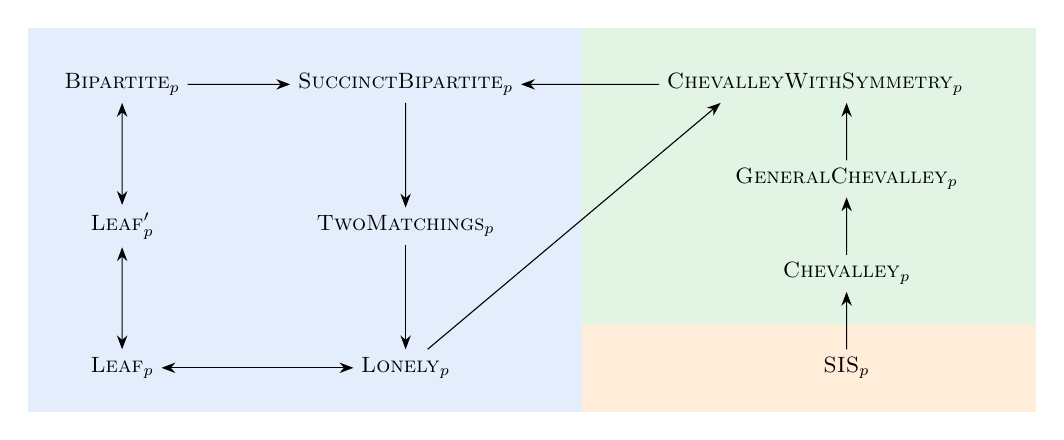
\begin{tikzpicture}[scale=0.8, transform shape]
	\def\hgap{2}
	\def\vgap{2.25}
	\draw[fill=Gblue!15, draw=none] (-7,2.4*\vgap) rectangle (1.8,-0.7);
	\draw[fill=Ggreen!15, draw=none] (9,2.4*\vgap) rectangle (1.8,-0.7);
	\draw[fill=orange!15, draw=none] (9,0.3*\vgap) rectangle (1.8,-0.7);
	\node (bip) at (-5.5,2*\vgap) {$\bipartite_p$};
	\node (leaf) at (-5.5,0) {$\leaf_p$};
	\node (leaf-p) at (-5.5,\vgap) {$\leaf'_p$};
	\node (lone) at (-1,0) {$\lonely_p$};
		\node (sbip) at (-1,2*\vgap) {$\sucBipartite_p$};
	\node (twomat) at (-1,\vgap) {$\twoMatchings_p$};

	\def\vgap{1.5}
	\node (combCh) at (5.5,4.5) {$\cChevalley_p$};
	\node (labelCh) at (6,4.5-\vgap) {$\lChevalley_p$};
	\node (Ch) at (6, 4.5-2*\vgap) {$\Chevalley_p$};
	\node (SIS) at (6, 4.5-3*\vgap) {$\sis_p$};

	\path[{Stealth[length=5pt]}-{Stealth[length=5pt]},line width=.4pt,black]
	(bip) edge (leaf-p)
	(leaf-p) edge (leaf)
	(leaf) edge (lone);

	\path[-{Stealth[length=5pt]},line width=.4pt,black]
	(bip) edge (sbip)
	(sbip) edge (twomat)
	(twomat) edge (lone)
	(lone) edge[bend right=0] ([shift={(-1.5,0)}]combCh.south)
	(combCh) edge (sbip)
	(labelCh) edge ([shift={(0.5,0)}]combCh.south)
	(Ch) edge (labelCh)
	(SIS) edge (Ch);
	\end{tikzpicture}
	\caption{Total search problems studied in this work. An arrow
	$A \rightarrow B$ denotes a reduction $A \reducible B$ that we establish.
	Problems in the \textcolor{Gblue}{blue} region are non-natural problems,
	which are all complete for $\PPA_p$. Problems in the
	\textcolor{Ggreen}{green} region are natural problems of which
	$\cChevalley_p$ is the one we show to be $\PPA_p$--complete. The problem
	in the \textcolor{orange}{orange} region is a cryptographically relevant problem.
				}
	\label{fig:ppa-landscape}
\end{figure}
 

\setcounter{section}{3}
\setcounter{theorem}{12}
\section{A Natural Complete Problem}
\label{sec:chevalley}





We start with some notation that will be useful for the
presentation of our results.
\smallskip

\paragr{Notations.} For any polynomial $g \in \bbF_p[\vecx]$, we
define $\deg(g)$ to be the degree of $g$. We define
\textit{the expansion to monic monomials} of $g$ as $\sum_{\ell = 1}^L t_{\ell}(\vecx)$, 
where $t_{\ell}(\vecx)$ is a monic monomial in
$\bbF_p[\vecx]$, i.e. a monomial with coefficient $1$. For example,
the expansion of the polynomial
$g(x_1, x_2) = x_1 \cdot (2 x_1 + 3 x_2)$ is
given by $x_1^2 + x_1^2 + x_1 x_2 + x_1 x_2 + x_1 x_2$.

For a polynomial system $\vec{f} := (f_1, \ldots, f_m) \in \bbF_p[\vecx]^m$, its affine variety $\calV_{\vecf} \subseteq \bbF_p^n$ is defined as
$\calV_{\vecf} \coloneqq \set{\vecx \in \bbF_p^n \mid \vecf(\vecx) = \vec{0}}$.
Let $\overline{\calV_{\vecf}} \coloneqq \bbF_p^n \setminus \calV_{\vecf}$. If the constant term of each $f_i$ is $0$, we say that $\vecf$ is {\em zecote}, standing for ``Zero Constant Term'' (owing to lack of known terminology and creativity on our part).

  
\subsection{The Chevalley-Warning Theorem} \label{sec:ChevalleyWarningProof}

  We repeat the formal statement of Chevalley-Warning Theorem together with its
proof.

\begin{cwthm}[\cite{r15,r37}]
    For any prime $p$ and a polynomial system
  $\vecf \in \bbF_p[\vecx]^m$ satisfying $\sum_{i = 1}^m \deg(f_i) < n$
  \emph{(CW Condition)}, $|\calV_{\vecf}| \equiv 0 \mod{p}$.
\end{cwthm}

  We describe the proof of \CWT through \autoref{lem:mainLemmaInProofOfCWT}.
Even though there are direct proofs, the following presentation helps motivate the generalizations we study in future sections. Given a polynomial system $\vecf \in
\bbF_p[\vecx]^m$, a key idea in the proof is the polynomial $\CW_{\vecf}(\vecx)
\coloneqq \prod_{i = 1}^m \CW_{f_i}(\vecx)$ where each $\CW_{f_i}(\vecx) := (1 - f_i(\vecx)^{p - 1})$. Observe that $\CW_{\vecf}(\vecx) = 1$ if
$\vecx \in \calV_{\vecf}$ and is $0$ otherwise. The following definition
describes the notion of a max-degree monomial of $\CW_{\vecf}$ that plays an important role in the proof.

\begin{definition}[\textsc{Max-Degree Monic Monomials}]
\label{def:max-degreeMonomial}
For any prime $p$, let $\vecf \in \bbF_p[\vecx]^m$ and let the expansion into monic monomials of $\CW_{f_i}(\vecx)$ be $\sum_{\ell = 1}^{r_i} t_{i, \ell}(\vecx)$. Let also $U_i = \{(i, \ell) \mid \ell \in [r_i]\}$ and $U = \bigtimes_{i = 1}^m U_i$, we define the following quantities.
  \begin{Enumerate}
    \item A \textit{monic monomial} of $\CW_{\vecf}$ is a product $t_S(\vecx) = \prod_{i = 1}^m t_{s_i}(\vecx)$ for $S = (s_1, \ldots, s_m) \in U$.
	    \item A \textit{max-degree monic monomial} of $\CW_{\vecf}$ is any monic monomial $t_S(\vecx)$, such that\\
    $t_S(\vecx) \equiv \prod_{j = 1}^n x_j^{p - 1} \mod{\set{x_i^p - x_i}_{i \in [n]}}$.
    \item We define $\calM_{\vecf}$ to be the set of max-degree monic monomials of $\CW_{\vecf}$, i.e. \\
	$\calM_{\vecf} \coloneqq \set{S \in U \mid t_S \text{ is a max-degree monic monomial of } \CW_{\vecf}}$.
  \end{Enumerate}
\end{definition}

\noindent In words, the monomials $t(S)$ are precisely the ones that arise when symbolically expanding $\CW_{\vecf}(\bx)$. We illustrate this with an example: Let $p = 3$ and $f_1(x_1, x_2) = x_1 + x_2$ and $f_2(x_1, x_2) = x_1^2$. Then modulo $\set{x_1^3 - x_1, x_2^3 - x_2}$, we have
\begin{align*}
\CW_{(f_1,f_2)}(x_1, x_2) &~=~ (1 - (x_1 + x_2)^2)(1 - (x_1^2)^2)\\
&~=~ (1 - x_1^2 - 2 x_1 x_2 - x_2^2) \cdot (1 - x_1^2)\\
&~=~ (1 + x_1^2 + x_1^2 + x_1x_2 +x_2^2 + x_2^2) \cdot (1 + x_1^2 + x_1^2)
\end{align*}

\noindent Thus there are $18$ $(= 6 \times 3)$ monic monomials in the system $(f_1, f_2)$. The monomial corresponding to $S = ((1,5),(2,2))$ is a maximal monomial since the $5$-th term in $\CW_{f_1}$ is $x_2^2$ and $2$-nd term in $\CW_{f_2}$ is $x_1^2$. Using the above definitions, we now state the main technical lemma of the proof of \CWT.

\begin{lemma}[Main Lemma in the proof of CWT] \label{lem:mainLemmaInProofOfCWT}
   For any prime $p$ and any system of polynomials
  $\vecf \in \bbF_p[\vecx]^m$, it holds that
  $\abs{\calV_{\vecf}} \equiv (-1)^n \abs{\calM_{\vecf}} \mod{p}$.
\end{lemma}

\begin{proof}
As noted earlier, $\CW_{\vecf}(\vecx) = 1$ if $\bx \in \calV_{\vecf}$ and is $0$ otherwise. Thus, it follows that $\abs{\calV_{\vecf}} \equiv \sum_{\bx \in \bbF_p^n} \CW_{\vecf}(\bx) \mod{p}$. For any monic monomial $m(\bx) = \prod_{j=1}^n x_j^{d_j}$, it holds that $\sum_{\bx \in \bbF_p^n} m(\bx) = 0$ if $d_j < p - 1$ for some $x_j$. On the other hand, for the monic max-degree monomial $m(\bx) = \prod_{j = 1}^n x_j^{p-1}$, it holds that $\sum_{\bx \in \bbF_p^n} m(\bx) = (p-1)^n$. Thus, we get that $|\calV_{\vecf}| \equiv \sum_{\bx \in \bbF_p^n} \CW_{\vecf}(\bx) \mod{p} \equiv \sum_{S\in U} \sum_{\bx \in \bbF_p^n} t_S(\vecx)  \mod{p} \equiv (-1)^n |\calM_{\vecf}| \mod{p}$.
\end{proof}

\noindent The proof of Chevalley-Warning Theorem follows easily from
\autoref{lem:mainLemmaInProofOfCWT}.

\begin{proof}[Proof of Chevalley-Warning Theorem.]
We have that $\deg(\CW_{\vecf}) \le (p - 1) \sum_{i = 1}^m \deg(f_i)$. Thus, if $\vecf$ satisfies \eqref{eq:CWcondition}, then $\deg(\CW_{\vecf}) < (p - 1) n$ and hence $\abs{\calM_{\vecf}} = 0$. \CWT now follows from \autoref{lem:mainLemmaInProofOfCWT}.
\end{proof}

\subsection{The Chevalley-Warning Theorem with Symmetry}
\label{sec:ChevalleyWarningWithSymmetry}

  In this section, we formalize the intuition that we built in
\hyperref[sec:proofsOfCancellation]{Sections~\ref{sec:proofsOfCancellation}} and \ref{sec:computationalChevalleyWarning} to prove the more general
statements to lead to the same conclusion as the Chevalley-Warning
Theorem.

  First, we prove a theorem that argues about the cardinality of $\calV_{\vecf}$
directly using some symmetry of the system of polynomials $\vecf$. Then,
combining this symmetry-based argument with the \eqref{eq:generalCWCondition} we get
the generalization of the Chevalley-Warning Theorem. Our natural
$\PPA_p$-complete problem is based on this generalization.

The theorem statements are simplified using the definition of
\textit{free action} of a group. For a permutation over $n$ elements $\sigma \in S_n$, we define
$\langle \sigma \rangle$ to be the sub-group generated by $\sigma$ and
$|\sigma|$ to be the order of $\langle\sigma \rangle$. For $\vecx \in \bbF_p^n$, $\sigma(\vecx)$ denotes the assignment obtained by permutating the variables of the assignment $\vecx$ according to $\sigma$.

\begin{definition}[\textsc{Free Group Action}]
    Let $\sigma \in S_n$ and $\calV \subseteq \bbF_p^n$, then we say that
  $\langle \sigma \rangle$ acts freely on $\calV$ if, for every
  $\vecx \in \calV$, it holds that $\sigma(\vecx) \in \calV$ and
  $\vecx \neq \sigma(\vecx)$.
\end{definition}

  Our first theorem highlights the
use of symmetry in arguing about the size of $\abs{\calV_{\vecf}}$.

\begin{theorem} \label{thm:symmetricChevalleyTheorem}
    Let $\vecf \in \F_p[\vecx]^m$ be a system of polynomials.
  If there exists a permutation $\sigma \in S_n$ with
  $\abs{\sigma} = p$ such that $\a{\sigma}$ acts freely on
  $\overline{\calV}_{\vecf}$, then $\abs{\calV_{\vecf}} \equiv 0 \mod{p}$.
\end{theorem}

\begin{proof}
    Since $\sigma$ acts freely on $\overline{\calV}_{\vecf}$, we can partition
  $\overline{\calV}_{\vecf}$ into orbits of any
  $\vecx \in \overline{\calV}_{\vecf}$ under actions of $\a{\sigma}$, namely
  sets of the type $\set{\sigma^i(\vecx)}_{i \in [p]}$ for
  $\vecx \in \overline{\calV}_{\vecf}$. Since $\a{\sigma}$ acts freely on
  $\overline{\calV}_{\vecf}$, each such orbit has size $p$. Thus, we can
  conclude that $\abs{\overline{\calV}_{\vecf}} \equiv 0 \pmod p$ from which
  the theorem follows.
\end{proof}

\begin{remark} \label{rem:syntacticVerificationOfSymmetry}
  For any polynomial system $\vecf$ and any
  permutation $\sigma$, we can check in linear time if $\abs{\sigma} = p$ and we
  can syntactically refute that $\langle \sigma \rangle$ acts freely on
  $\overline{\calV}_{\vecf}$ with an $\vecx \in \bbF_p^n \smallsetminus \set{\vec{0}}$ such that $\vecf(\sigma(\vecx)) = \vec{0}$ or $\sigma(\vecx) = \vecx$.
\end{remark}
\bigskip

We now state and prove an extension of \CWT that captures both
the argument from \autoref{lem:mainLemmaInProofOfCWT} and the symmetry
argument from \autoref{thm:symmetricChevalleyTheorem}.

\begin{theorem}[\textsc{Chevalley-Warning with Symmetry Theorem}]
\label{thm:combinedChevalleyTheorem}
	  Let $\vecg \in \F_p[\vecx]^{m_g}$ and
	$\vech \in \F_p[\vecx]^{m_h}$ be two systems of polynomials, and
	$\vecf \coloneqq (\vecg, \vech)$. If there exists a permutation $\sigma \in S_n$ with $\abs{\sigma} = p$ such that (1) $\calM_{\vecg} = \emptyset$ and (2) $\a{\sigma}$ acts freely on
	$\calV_{\vecg} \cap \overline{\calV_{\vech}}$, then $\abs{\calV_{\vecf}} = 0 \mod{p}$.
\end{theorem}

\begin{remark} \label{rem:conditionsOfChevalleyWithSymmetry}
    We point to the special form of Condition 2. By definition,
  $\calV_{\vecf} = \calV_{\vecg} \cap \calV_{\vech}$, hence if $\a{\sigma}$
  were to act freely on $\overline{\calV_{\vecg}} \cup \overline{\calV_{\vech}}$ (or even $\calV_{\vecg} \cap \calV_{\vech}$), then we could just
  use \autoref{thm:symmetricChevalleyTheorem} to get that
  $\abs{\calV_{\vecf}} \equiv 0 \mod{p}$. In the above theorem,
  we only require that $\a{\sigma}$ acts freely on
  $\calV_{\vecg} \cap \overline{\calV_{\vech}}$. Observe that
  \autoref{thm:symmetricChevalleyTheorem} follows as a special case of \CWT with
  Symmetry by setting $m_g = 0$. Additionally, by setting $m_h = 0$ we get the generalization of \CWT corresponding to the
  \eqref{eq:generalCWCondition} as presented in
  \autoref{sec:computationalChevalleyWarning}.
\end{remark}

\begin{proof}[Proof of \autoref{thm:combinedChevalleyTheorem}]
  	If $\CW_{\vecg}$ does not have any max-
	degree monic monomials, we have $\abs{\calV_{\vecg}} \equiv 0 \mod{p}$ (similar to proof of \CWT) and, since
	$\overline{\calV_{\vecg}} = \F_p^n \setminus \calV_{\vecg}$, we have $\abs{\overline{\calV_{\vecg}}} \equiv 0 \mod{p}$. Also,
	since $\a{\sigma}$ acts freely on $\calV_{\vecg} \cap
	\overline{\calV_{\vech}}$, we have
	$\abs{\calV_{\vecg} \cap \overline{\calV_{\vech}}} \equiv 0 \mod{p}$ (similar to the proof of
	\autoref{thm:symmetricChevalleyTheorem}). Hence,
	$\abs{\overline{\calV_{\vecf}}} = \abs{\overline{\calV_{\vecg} \cap
	\calV_{\vech}}}  = \abs{\overline{\calV_{\vecg}} \cup
	\overline{\calV_{\vech}}} = \abs{\overline{\calV_{\vecg}}} +
	\abs{\calV_{\vecg} \cap \overline{\calV_{\vech}}} \equiv  0 \mod{p}$. Thus,
	$\abs{\calV_{\vecf}} \equiv 0 \mod{p}$.
\end{proof}

\subsection{Computational Problems Related to Chevalley-Warning Theorem}
\label{sec:computationalChevalleyWarningFormal}

  We now follow the intuition developed in the previous section and in
\autoref{sec:intro-complete} to formally define the computational problems
$\eChevalleyp$, $\lChevalleyp$, and $\cChevalleyp$.
\medskip


	\noindent
	\begin{minipage}{\linewidth}
		\begin{definition}
			\label{def:explicit-chevalley} \contour{black}{($\eChevalleyp$)}\vspace{-5pt}
			\begin{itemize}[leftmargin=2.15cm,itemsep=4pt]
				\item[\slshape Principle:] Chevalley-Warning Theorem.
				\item[\slshape Input:] $\vecf \in \bbF_p[\vecx]^m$ : an explicit zecote polynomial system.
				\item[\slshape Condition:] $\sum_{i = 1}^m \deg(f_i) < n$.
				\item[\slshape Output:] $\vecx \in \bbF_p^n$ such that $\vecx \neq \vec{0}$ and $\vecf(\vecx) = \vec{0}$.
			\end{itemize}
		\end{definition}
	\end{minipage}\vspace{3mm}

\bigskip


	\noindent
	\begin{minipage}{\linewidth}
		\begin{definition}
			\label{def:general-chevalley} \contour{black}{($\lChevalleyp$)}\vspace{-5pt}
			\begin{itemize}[leftmargin=2.15cm,itemsep=4pt]
				\item[\slshape Principle:] General Chevalley-Warning Theorem via \eqref{eq:generalCWCondition}.
				\item[\slshape Input:] $\vecf \in \bbF_p[\vecx]^m$ : an explicit zecote polynomial system.
				\item[\slshape Output:] \begin{Enumerate}[leftmargin=*]
  \item[0.] A max-degree monic monomial $t_S(\vecx)$ of $\CW_{\vecf}$, or
  \item $\vecx \in \bbF_p^n$ such that $\vecx \neq \vec{0}$ and $\vecf(\vecx) = \vec{0}$.
\end{Enumerate}
			\end{itemize}
		\end{definition}
	\end{minipage}\vspace{3mm}


\bigskip


	\noindent
	\begin{minipage}{\linewidth}
		\begin{definition}
			\label{def:combined-chevalley} \contour{black}{($\cChevalleyp$)}\vspace{-5pt}
			\begin{itemize}[leftmargin=2.15cm,itemsep=4pt]
				\item[\slshape Principle:] Chevalley-Warning Theorem with Symmetry (\autoref{thm:combinedChevalleyTheorem}).
				\item[\slshape Input:] $\triangleright$ $\vecg \in \bbF_p[\vecx]^{m_g}$ and $\vech \in \bbF_p[\vecx]^{m_h}$ : explicit zecote polynomial systems\\
 $\triangleright$ $\sigma \in S_n$ : a permutation over $[n]$.
				\item[\slshape Condition:] $|\sigma| = p$.
				\item[\slshape Output:] \begin{Enumerate}[leftmargin=*]
  \item[0.] (a) A max-degree monic monomial $t_S(\vecx)$ of $\CW_{\vecg}$, or
  \item[] (b) $\vecx \in \calV_{\vecg} \cap \overline{\calV_{\vech}}$ such that
        $\sigma(\vecx) \not\in (\calV_{\vecg} \cap \overline{\calV_{\vech}}) \smallsetminus \set{\vecx}$, or
  \item $\vecx \in \bbF_p^n$ such that $\vecx \neq \vec{0}$ and $\vecf(\vecx) = \vec{0}$.
\end{Enumerate}
			\end{itemize}
		\end{definition}
	\end{minipage}\vspace{3mm}


\begin{remark} \label{rem:computationalDefinitions}
    Some observations about the above computational problems follow:
  \begin{Enumerate}
    \item In the problems $\lChevalleyp$ and $\cChevalleyp$,  we assume that, if the output is a max-degree monic monomial, this is given via the multiset of indices $S$ that describes the monomial as formalized in \autoref{def:max-degreeMonomial}.
    \item We have $\eChevalleyp \preceq \lChevalleyp \preceq \cChevalleyp$. Thus, inclusion of $\cChevalleyp$ in $\PPA_p$ implies that the problems $\eChevalleyp$ and $\lChevalleyp$ are in $\PPA_p$. Also, in Section6 we prove that $\sis_p \preceq \eChevalleyp$, where $\sis_p$ is a cryptographically relevant problem. This shows that the $\lChevalleyp$ and the $\cChevalleyp$ problems are at least as hard as the $\sis_p$ problem.
  \end{Enumerate}
\end{remark}

\noindent We restate our main result.

\completeness*

\subsection{\boldmath $\cChevalleyp$ is $\PPAp$--complete}
\label{sec:proofOfCombinedChevalley}

  We fist prove that $\cChevalley$ is in $\PPAp$ and then
prove its $\PPAp$-hardness.


\subsubsection{\boldmath $\cChevalleyp$ is in $\PPA_p$}

Even though Papadimitriou~\cite{r33} provided a rough proof sketch of $\Chevalley_p \in \PPAp$, a formal proof was not given. We show that $\cChevalleyp$ is in $\PPAp$ (and so are $\lChevalleyp$ and $\eChevalleyp$). In order to do so we extend the definition of $\bipartiteq$ to instances where the vertices might have exponential degree and edges appear with multiplicity. The key here is to define a $\bipartite_q$ instance with unbounded (even exponential) degree, but with additional information that allows us to verify solutions efficiently.\\[-1mm]


\noindent
\begin{minipage}{\linewidth}
\begin{definition}
	\label{def:succ-bipartite} \contour{black}{($\sucBipartite_q$)}\vspace{-5pt}
	\begin{itemize}[leftmargin=2.15cm,itemsep=4pt]
		\item[\slshape Principle:] Similar to $\bipartite_q$, but degrees are allowed to be exponentially large, edges are allowed with multiplicities at most $q-1$.
		\item[\slshape Object:] Bipartite graph $G = (V \cup U, E)$ s.t. $E \subseteq V \times U \times \bbZ_q$. Designated edge $e^* \in E$.
		\item[\slshape Inputs:] Let $V \coloneqq \set{0} \times \bit^{n-1}$ and $U \coloneqq \set{1} \times \bit^{n-1}$:\\
	$\triangleright$ $\calC:V \times U \to [q]$, edge counting circuit\\
	$\triangleright$ $\phi_V: V \times U \times [q] \to (U \times [q])^{q}$, grouping pivoted at $V$\\
	$\triangleright$ $\phi_U: V \times U \times [q] \to (V \times [q])^{q}$, grouping pivoted at $U$\\
	$\triangleright$ $e^* = (v^*, u^*, k^*)$, designated edge
		\item[\slshape Encoding:] $V \coloneqq \set{0} \times \bit^{n-1}$, $U \coloneqq \set{1} \times \bit^{n-1}$,\\
	$E \coloneqq \set{(v,u,k) : 1 \le k \le C(v,u),\ (v,u) \in V \times U}$ (here $k$ distinguishes multiplicities)\\
	Edge $(v,u,k)$ is grouped with $\set{(v, u', k') : (u',k') \in \phi_V(v,u,k)}$ (pivoting at $v$),\\
	\hspace*{1cm} provided $|\phi_V(v,u,k)| = q$, all $(v,u',k') \in E$ and $\phi_V(v,u',k') = \phi_V(v,u,k)$.\\
	Edge $(v,u,k)$ is grouped with $\set{(v', u, k') : (v',k') \in \phi_U(v,u,k)}$ (pivoting at $u$),\\
	\hspace*{1cm} provided $|\phi_U(v,u,k)| = q$, all $(v,u',k') \in E$ and $\phi_U(v',u,k') = \phi_V(v,u,k)$.
		\item[\slshape Solutions:] $e^*$ if $e^*$ is grouped, pivoting at $v^*$, or if $e^*$ is not grouped pivoting at $u^*$, OR\\
	$e \ne e^*$ if $e$ is not grouped pivoting at one of its ends.
	\end{itemize}
\end{definition}
\end{minipage}\vspace{5mm}

In words, $\sucBipartite_p$ encodes a bipartite graph with arbitrary degree. Instead of listing the neighbors of a vertex using a circuit, we have a circuit that outputs the multiplicity of edges between any two given vertices. We are therefore unable to efficiently count the number of edges incident on any vertex. The grouping function $\phi_V$ aims to group edges incident on any vertex $v \in V$ into groups of size $q$. Similarly, $\phi_U$ aims to group edges incident on any vertex $u \in U$. The underlying principle is that if we have an edge $e^*$ that is not grouped pivoting at $v^*$ (one of its endpoints), then either $e^*$ is not pivoted at $u^*$ (its other endpoint) or there exists another edge that is also not grouped pivoting at one of its ends. Note that in contrast to the problems previously defined, $v^*$ might still be an endpoint of a valid solution.

\begin{lemma} \label{lem:combinedChevalleyPPAp}
 For all primes $p$, $\cChevalleyp \in \PPAp$.
\end{lemma}
\begin{proof}We reduce $\cChevalleyp$ to $\sucBipartite_p$, which we show to be $\PPA_p$--complete in \autoref{sec:sucBipartite}. Given an instance of $\cChevalleyp$, namely a zecote polynomial system $\vecf = (\vecg, \vech)$ and a permutation $\sigma$, we construct a bipartite graph $G = (U \cup V, E)$ encoded as an instance of $\sucBipartite_p$ as follows. 

 \paragraph{Description of vertices.} $U = \bbF_p^n$, namely all possible assignments
 of $\vecx$. The vertices of $V$ are divided into two parts $V_1 \cup V_2$.
 The part $V_1$ contains one vertex for each monomial in the expansion of $\CW_{\vecg} = \prod_{i = 1}^{m_g} (1 - g_i^{p-1})$. Since $p$ is constant, we can
 efficiently list out the monomials of $1 - g_{i}^{p-1}$. For a fixed lexicographic ordering of the
 monomials of each $\CW_{g_i} \coloneqq 1 - g_{i}^{p-1}$, a
 monomial of $\CW_{\vecg}$ is represented by a tuple
 $(a_1, a_{2}, \dots, a_{m_g})$ with $0 \leq a_{i} < L_{i}$, where
 $a_{i}$ represents the index of a monomial of $\CW_{g_i}$ and  $L_{i}$
 is the number of monomials of $\CW_{g_i}$, where $a_i = 0$ corresponds to the constant term $1$. The part $V_2 \coloneqq \binom{\bbF_p^n}{p}$, i.e. it contains a vertex for each subset of $p$ distinct elements in $\bbF_p^n$.


 \paragraph{Description of edges.} We first describe the edges between $U$ and $V_1$, namely include an
 edge between an assignment $\vecx$ and a monomial $t$ with
 multiplicity $t(\vecx)$. With these edges in place, the degree of vertices are as follows:\vspace{-2mm}
 \begin{itemize}[leftmargin=0.5cm]
	\item $\vecx = 0^n$ has a single edge corresponding to the constant monomial $1$, since $\vecf$ is zecote. We let this be the designated edge $e^*$ in the final $\sucBipartite_p$ instance.
	\item $\vecx \notin \calV_{\vecg}$ has $0 \pmod p$ edges
	(counting multiplicities). Since $\CW_{\vecg}(\vecx) = 0$, the sum over all monomials of $t(\vecx)$ must be $0 \mod{p}$.
	\item $\vecx \in \calV_{\vecg}$ has $1 \pmod p$ edges (counting multiplicities), since the sum over all $t(\vecx)$ monomials gives $\CW_{\vecg}(\bx) \equiv 1 \mod{p}$.
 \end{itemize}
 Thus with the edges so far, the vertices (excluding $0^n$), with degree $\not\equiv 0 \mod{p}$ are precisely vertices  $t \in V_1$ such that $\sum_{\vecx} t(\vecx) \not\equiv 0 \pmod p$ or $\vecx \in \calV_{\vecg} \smallsetminus \set{0^n}$. For the former case, if $t$ contained a variable with degree less than $p-1$, then $\sum_{\vecx} t(\vecx) \equiv 0 \pmod p$. Hence, it must be that $t = \prod\limits_{i = 1}^{ n} x_i^{p-1}$. In the later case, the degree of $\vecx $ is $1 \mod{p}$ and hence $\vecx \in \calV_{\vecg}$. 
 However, there is no guarantee that a vertex $\vecx$ with degree $1 \mod{p}$ is in $\calV_{\vech}$ as well. To argue
 about $\vech$, we add edges between $U$ and $V_2$ that exclude solutions $\vecx \in \calV_{\vecg} \cap \overline{\calV_{\vech}}$, on which $\sigma$ acts freely (that is, $\sigma(\vecx) = \vecx$). More specifically, for
 $\vecx \in \calV_{\vecg} \cap \overline{\calV_{\vech}}$, if $\sigma(\vecx) \ne \vecx$,
  we add an edge with multiplicity $p-1$ between $\vecx$ and $\Sigma_{\vecx} \in V_2$ where $\Sigma_{\vecx} \coloneqq \{\sigma^i(\vecx)\}_{i \in \bbZ_p}$ (note that, in this case $\abs{\Sigma_{\vecx}} = p$ since $\sigma(\vecx) \ne \vecx$ and $|\sigma| = p$ is prime).
 Observe that, if a vertex in $V_2$ corresponds
 to a $\Sigma_{\vecx}$, it has $p$ edges each with multiplicity $p-1$, one for each
 $\vecx' \in \Sigma_{\vecx}$ only if $\Sigma_{\vecx} \subseteq \calV_{\vecg} \cap \overline{\calV_{\vech}}$. If a vertex in $V_2$ does not correspond to a
 $\Sigma_{\vecx}$, then it has no edges. Thus, a vertex in $V_2$ has degree $\not\equiv 0 \mod{p}$ iff it contains an $\vecx \in \calV_{\vecg} \cap \overline{\calV_{\vech}}$ such that $\sigma(\vecx) \notin \calV_{\vecg} \cap \overline{\calV_{\vech}}$.

 Thus, with all the edges added, vertices with degree $\not\equiv 0 \mod{p}$ correspond to one of\vspace{-2mm}
 \begin{itemize}
 \item $\vecx \in \calV_{\vecg} \cap \calV_{\vech}$ such that $\vecx \ne \vec{0}$, or
 \item $t \in V_1$ such that $t(\vecx)$ is a max-degree monomial or
 \item $\vecx \in \calV_{\vecg} \cap \overline{\calV_{\vech}}$ such that $\sigma(\vecx) = \vecx$ or
 \item $v \in V_2$ such that $\exists\, \vecx \in v$ satisfying $\vecx \in \calV_{\vecg} \cap \overline{\calV_{\vech}}$ and $\sigma(\vecx) \notin \calV_{\vecg} \cap \overline{\calV_{\vech}}$.
 \end{itemize}
 These correspond precisely to the solutions of $\cChevalleyp$. To summarize, the edge
 counting circuit $C$ on input $(\vecx, t) \in U \times V_1$ outputs
 $t(\vecx)$ and on input $(\vecx, v) \in U \times V_2$ outputs $p-1$ if
 $\vecx \in \calV_{\vecg} \cap \overline{\calV_{\vech}}$, $\sigma(\vecx) \ne \vecx$ and $v = \Sigma_{\vecx}$ and 0
 otherwise.


 \paragraph{Grouping Functions.}
      The grouping functions $\phi_U$ and $\phi_V$ are defined as follows (analogous to the so-called ``chessplayer algorithm'' in \cite{r33}):
 \begin{itemize}[label=$\triangleright$,leftmargin=0.5cm]
	\item Grouping $\phi_U$ (corresponding to endpoint in $U$):
\begin{itemize}[leftmargin=0.25cm]
		\item For $\vecx \in \overline{\calV_{\vecg}}$: there exists some $i$ such
		that $\CW_{g_i}(\vecx) = 0$. Consider an edge
		$(\vecx,(a_1,a_2, \dots, a_{m_g}),k)$. We can explicitly list out the multiset containing the monomials
		$t_j = (a_1,a_2, \dots, a_i \gets j, \dots, a_{m_g})$ with multiplicity
	        $t_j(\vecx)$, for each $1 \le j \le L_i$. Since $\CW_{g_i}(\vecx) = 0$, this multiset has size
		multiple of $p$. Hence, we can canonically divide its elements into groups of
		size $p$, counting multiplicities and $\phi_U$ returns the subset containing $(t,k)$.
		\item For $\vecx \in \calV_{\vecg} \cap \overline{\calV_{\vech}}$ such that $\sigma(\vecx) \ne \vecx$: Note that $g_{i}^{p-1}(\vecx) = 0$ for all $i \in \bracks{m_g}$.
		Let $v_1 \in V_1$ be the vertex corresponding to the
		constant monomial $1$. $\phi_U$ groups the edge $(\vecx, v_1, 1)$ (of multiplicity $1$) with the $p-1$ edges $(\vecx, \Sigma_{\vecx}, k)$ for $k \in [p-1]$.
		For any other $t \in  V_1 \setminus \set{v_1}$ and an edge $(\vecx, t,k)$, we have that
		$t = (a_1,\dots, a_{m_g})$ has $a_i \ne 0$ for some $i$. We define
		the multiset containing $t_j = (a_1, \dots, a_{i} \gets j, \dots a_{m_g})$
		with multiplicity $t_j(\vecx)$ for each $1 \le j < L_i$. Since
		$g_{i}^{p-1}(\vecx) = 0$, this multiset has size which is a multiple of $p$, which we can canonically partition into groups of size $p$. Thus, $\phi_U$ on input
		$(\vecx, t, k)$ returns the group containing $(t,k)$.
 	\end{itemize}
	\item Grouping $\phi_V$ (corresponding to endpoint in $V$):
		\begin{itemize}[leftmargin=0.25cm]
		\item For $t \in V_1$ such that $t \neq \prod\limits_{i = 1}^n x_i^{p-1}$:
		there exists a variable $x_i$ with degree less than $p-1$. For
		$\vecx_j = (x_1, \dots, x_{i-1}, x_i \gets j, \dots, x_n)$ with $j \in \bbF_p$
		we define the multiset $\set{(\vecx_j, t(\vecx_j))}_{j \in \bbF_p}$.
		Since $\sum\limits_{j = 0}^{p-1} t(\vecx_j) = 0$, this multiset has
		size multiple of $p$, so we can canonically partition it into groups of size $p$. Then,
		$\phi_V(\vecx, t, k)$ returns the group containing $(\vecx,k)$,
		\item For $v \in V_2$: if $\deg(v) = 0$, then there is no grouping to be done. Else if $\deg(v) \equiv 0 \mod{p}$ then $\phi_V(\vecx,t,k)$ returns
          		$\set{(\vecx,k)}_{\vecx \in v}$.
	  \end{itemize}
\end{itemize}
	Thus, for any vertex with degree $\equiv 0 \mod{p}$, we have provided a grouping function for all its edges. So, for any edge that is not grouped by grouping function at any of its endpoints, then such an endpoint must have degree $\not\equiv 0 \mod{p}$ and hence point to a valid solution of the $\cChevalleyp$ instance.
\end{proof}



\subsubsection{$\cChevalleyp$ is $\PPA_p$--hard}

We show that $\lonely_p \preceq \cChevalleyp$. In the $\cChevalleyp$ instance that we create, we will ensure that there are no solutions of type 0 (as in \autoref{def:combined-chevalley}) and thus, the only valid solutions will be of type 1. In order to do so, we introduce the notions of labeling and proper labeling and prove a generalization of \CWT that we call Labeled \CWT (\autoref{thm:labeledChevalleyWarningTheorem}).

As we will see, the Labeled \CWT, is just a
re-formulation of the original \CWT rather than a generalization. To
understand the Labeled \CWT we start with some
examples that do not seem to satisfy the Chevalley-Warning
condition, but where a solution exists.

\bigskip
\paragr{Example 1.} Consider the case where $p = 3$ and
$f(x_1, x_2) = x_2 - x_1^2$. In this case the Chevalley-Warning condition is not met, since we have $2$ variables and the total degree is also
$2$. But, let us consider a slightly different polynomial where we
replace the variable $x_2$ with the product of two variables
$x_{21}, x_{22}$ then we get the polynomial
$g(x_1, x_{21}, x_{22}) = x_{21} \cdot x_{22} - x_1^2$. Now,
$g$ satisfies \eqref{eq:CWcondition} and hence, we
conclude that the number of roots of $g$ is a multiple of $3$.
Interestingly, from this fact we can argue that there exists a non-trivial solution for $f(\vecx) = 0$.
In particular, the assignment $x_1 = 0$, $x_2 = 0$ corresponds to five
assignments of the variables $x_1$, $x_{21}$, $x_{22}$. Hence, since
$\abs{\calV_{g}} = 0 \mod{3}$, $g$ has another root, which corresponds to a
non-trivial root of $f$. In this example, we applied the
\CWT on a slightly different polynomial than $f$
to argue about the existence of non-trivial solutions of $f$, even though $f$ did not satisfy \eqref{eq:CWcondition} itself.
\bigskip

\paragr{Ignore Some Terms.} The Labeled \CWT formalizes the phenomenon
observed in Example 1 and shows that under certain conditions we can
\textit{ignore some terms} when defining the degree of each polynomial.
For instance, in Example 1, we can ignore the term
$x_1^2$ when computing the degree of $f$ and treat $f$ as a degree $1$
polynomial of $2$ variables, in which case the condition of \CWT is
satisfied.

We describe which terms can be ignored by defining a \textit{labeling}
of the terms of each polynomial in the system. The labels take values in
$\{-1, 0, +1\}$ and our final goal is to ignore the terms with label
$+1$. Of course, it should not be possible to define any labeling that
we want; for example we cannot ignore all the terms of a polynomial.
Next, we describe the rules of a \textit{proper labeling} that will
allow us to prove the Labeled \CWT. We start with
a definition of a labeling.

\begin{definition}[\textsc{Monomial Labeling}]
  \label{def:monomiallabeling}
     Let $\vecf \in \bbF[\vecx]^m$ and let $t_{i j}$ be the $j$-th monomial of the polynomial $f_i \in \bbF[\vecx]$ (written in some canonical sorted order). Let $\calT$ be the
  set of all pairs $(i, j)$ such that $t_{i j}$ is a monomial in
  $\vecf$. A \textit{labeling} of $\vecf$ is a function
  $\lambda : \calT \to \{-1, 0, +1\}$ and we say that $\lambda(i, j)$
  is the \textit{label} of $t_{i j}$ according to $\lambda$.
\end{definition}

\begin{definition}[\textsc{Labeled Degree}] \label{def:labeledDegree}
    For $\vecf \in \bbF[\vecx]^m$ with a labeling $\lambda$,     we define the \textit{labeled degree} of $f_i$ as,
      $ \deg^{\lambda}(f_i)\coloneqq \max_{j\,:\,\lambda(i, j) \ne +1} \deg(t_{i j})$, in words, maximum degree among monomials of $f_i$ labeled either $0$ or $-1$.
\end{definition}

\paragr{Example 1 (continued).} According to the lexicographic ordering,
$f(x_1, x_2) = - x_1^2 + x_2$ and we have the monomials
$t_{1 1} = - x_1^2$ and $t_{1 2} = x_2$. Hence, one possible labeling,
which as we will see later corresponds to the vanilla Chevalley-Warning
Theorem, is $\lambda(1, 1) = \lambda(1, 2) = 0$. According to this labeling,
$\deg^{\lambda}(f) = 2$. Another possible
labeling, that, as we will see, allows us to apply the Labeled
\CWT\!, is $\lambda(1, 1) = +1$ and $\lambda(1, 2) = -1$.
In this case, the labeled degree is $\deg^{\lambda}(f) = 1$.
\bigskip

  As we highlighted before, our goal is to prove the Chevalley-Warning
Theorem, but with the weaker condition that
$\sum_{i = 1}^m \deg^{\lambda}(f_{i}) < n$ instead of
$\sum_{i = 1}^m \deg(f_i) < n$. Of course, we first have to restrict the
space of all possible labelings by defining {\em proper labelings}.
In order to make the condition of proper labelings easier to interpret
we start by defining the notion of a labeling graph.

\begin{definition}[\textsc{Labeling Graph}] \label{def:labelingGraph}
  For $\vecf \in \bbF[\vecx]^m$ with a labeling $\lambda$, we define the
  \textit{labeling graph} $G_{\lambda} = \p{U \cup V, E}$ as a
  directed bipartite graph on vertices
  $U = \set{x_1, \dots, x_n}$ and $V=\set{f_1, \dots, f_m}$. The edge
  $(x_j \to f_i)$ belongs to $E$ if $x_j$ appears in a monomial
  $t_{i r}$ in $f_i$ with label $+1$, i.e. $\lambda(i, r) = +1$. Symmetrically, the edge
  $(f_i \to x_j)$ belongs to $E$ if the $x_j$ appears in a monomial
  $t_{i r}$ in $f_i$ with label $-1$, i.e. $\lambda(i, r) = -1$.
\end{definition}

\paragr{Example 2.} Let $p = 2$ and
$f_1(x_1, x_2, x_3, x_4) = x_1 x_2 - x_3$,
$f_2(x_1, x_2, x_3, x_4) = x_1 x_3 - x_4$. In this system, if we use the
lexicographic monomial ordering we have the monomials
$t_{1 1} = x_1 x_2$,
$t_{1 2} = - x_3$, $t_{2 1} = x_1 x_3$, $t_{2 2} = - x_4$. The following
figure shows the graph $G_{\lambda}$ for the labeling
$\lambda(1, 1) = +1$, $\lambda(1, 2) = -1$, $\lambda(2, 1) = +1$ and
$\lambda(2, 2) = -1$.

\begin{center}
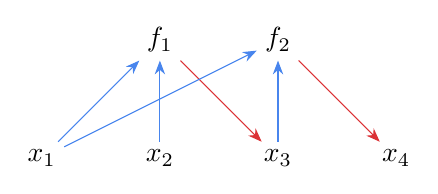
\begin{tikzpicture}
	\tikzset{
		inner sep=0,outer sep=3,
		neg/.style={color=Gred},
		posi/.style={color=Gblue}}
	\def\hgap{1.5}
	\def\vgap{1.5}
	\node (f1) at (0,\vgap) {$f_1$};
	\node (f2) at (\hgap,\vgap) {$f_2$};

	\node (x1) at (-\hgap,0) {$x_1$};
	\node (x2)at (0,0) {$x_2$};
	\node (x3) at (\hgap,0) {$x_3$};
	\node (x4) at (2*\hgap,0) {$x_4$};

	\path[-{Stealth[length=5pt]},line width=.4pt,black]
	(f1) edge[neg] (x3)
	(f2) edge[neg] (x4)
	(x1) edge[posi] (f1)
	(x2) edge[posi] (f1)
	(x1) edge[posi] (f2)
	(x3) edge[posi] (f2);
\end{tikzpicture}
\end{center}


\begin{definition}[\textsc{Proper Labeling}] \label{def:properLabel}
  Let $\vecf \in \bbF[\vecx]^m$ with a labeling $\lambda$.
    We say that the labeling $\lambda$ is \textit{proper} if the following
  conditions hold.\\[-6mm]
  \begin{enumerate}
    \item[(1)] For all $i$, either $\lambda(i, j) \in \set{-1, 1}$ for all $j$, or $\lambda(i, j) = 0$ for all $j$.
    \item[(2)] If two monomials $t_{i j}$, $t_{i j'}$ contain the same
          variable $x_k$, then $\lambda(i, j) = \lambda(i, j')$.
    \item[(3)] If $\lambda(i, j) = -1$, then $t_{i j}$ is multilinear.
    \item[(4)] If $x_k$ is a variable in the monomials
          $t_{i j}$, $t_{i' j'}$,
          with $i \neq i'$ and $\lambda(i, j) = -1$, then
          $\lambda(i', j') = +1$.
    \item[(5)] If $\lambda(i, j) \neq 0$, then there exists a $j'$ such that
          $\lambda(i, j') = -1$.
    \item[(6)] The labeling graph $G_{\lambda}$ contains no directed cycles.
  \end{enumerate}
\end{definition}

\noindent We give an equivalent way to understand the definition of a proper labeling.
\begin{itemize}[label=$\triangleright$]
\item Condition (1) : there is a partition of the polynomial system $\vecf$ into polynomial systems $\vecg$ and $\vech$ such that all monomials in $\vecg$ are labeled in $\set{+1, -1}$ and all monomials in $\vech$ are labeled $0$.
\item Condition (2) : each polynomial $g_i$ in $\vecg$ can be written as $g_i = g_i^+ + g_i^{-}$, such that $g_i^+$ and $g_i^-$ are polynomials on a disjoint set of variables.
\item Condition (3) : Each $g_i^-$ is multilinear.
\item Condition (4) : Any variable $x_k$ can appear in at most one of the $g_i^-$. Moreover, if an $x_k$ appears in some $g_i^-$, it does not appear in any $h_j$ in $\vech$.
\item Condition (5) : Every $g_i^-$ involves at least one variable.
\item Condition (6) : The graph $G_{\lambda}$ is essentially between polynomials in $\vecg$ and the variables that appear in them, with an edge $(g_i \to x_k)$ if $x_k$ appears in $g_i^-$ or an edge $(x_k \to g_i)$ if $x_k$ appears in $g_i^+$.
\item Note that $\deg^\lambda(g_i) = \deg(g_i^-)$, whereas $\deg^\lambda(h_j) = \deg(h_j)$.
\end{itemize}

\noindent It is easy to see that the trivial labeling $\lambda(i, j) = 0$ is always proper.
As we will see this special case of the Labeled \CWT\! corresponds to the
original \CWT\!. Note that in this case the
labeling graph $G_{\lambda}$ is an empty graph. Also, given a
system of polynomials $\vecf$ and a labeling $\lambda$, it is possible to
check in polynomial time whether the labeling $\lambda$ is proper or not.

\bigskip
\paragr{Example 2 (continued).} It is an instructive exercise to verify that the labeling $\lambda$ specified was indeed a proper labeling of $\vecf$.
\bigskip


\begin{theorem}[\textsc{Labeled Chevalley-Warning Theorem}]
  \label{thm:labeledChevalleyWarningTheorem}
    Let $\F_q$ be a finite field with characteristic $p$ and
  $\vecf \in \F_q[\vecx]^m$. If $\lambda$ is a proper labeling of
  $\vecf$ with $\sum_{i = 1}^m \deg^{\lambda}(f_i) < n$, then $|\calM_{\vecf}| = 0$. In particular, $\abs{\calV_{\vecf}} \equiv 0 \mod{p}$.
\end{theorem}
\begin{proof}
We can re-write $\CW_{\vecf}(x)$ as
$\sum_{S \subseteq [m]} \prod_{i \in S} (-1)^{|S|} f_i^{p-1}$.
We'll show that every monomial appearing in the expansion of
$\prod_{i \in S} f_i^{p-1}$ will have at least one variable with degree at most
$p-1$. For simplicity, we focus on the case $S = [m]$ and the other cases of
$S$ follow similarly.

We index a monomial of $\prod_{i \in [m]} f_i^{p-1}$ with a tuple
$((j_{11},j_{12}, \dots, j_{1(p-1)}), \dots, (j_{m1}, \dots, j_{m(p-1)}))$ with
$1 \leq j_{i\ell} \leq L_{i}$ where $L_i$ is the number of monomials in the
explicit representation of $f_i$.
The coordinates $(j_{i1}, \dots, j_{i(p-1)})$ represent the indices of the
monomials chosen from each of the $p-1$ copies of $f_i^{p-1}$. More succinctly,
we have $t = \prod_{i=1}^m \prod_{\ell=1}^{p-1} t_{i,j_{i\ell}}$.\\[-0.8mm]

\noindent {\em Case 1. $\lambda(i,j_{i\ell}) \in \set{0, -1}$, for all $(i,\ell)$:}\\
Here, $\deg(t) \le (p-1) \sum_{i=1}^m \deg^{\lambda}(f_i)$ which, by our assumption, is strictly less than $(p-1)n$. Hence, there is a variable with degree less than $p-1$.\\[-0.8mm]

\noindent {\em Case 2. There is a unique $i$ with $\lambda(i,j_{i\ell}) = +1$ for some $\ell$:} (warmup for case 3)\\
That is, for all $i'\neq i$, $\lambda(i',j_{i'\ell})  \in \set{0, -1}$. By condition (5) of proper labeling there exists a $j' \neq j_{i\ell}$ such that  $\lambda(i,j') = -1$. Let $x_k$ be a variable in the monomial $t_{ij'}$. By condition (2), $x_k$ is not present in the monomial $t_{i,j_{i\ell}}$ and by condition (3), its degree in $(t_{i,j_{i,1}}, \dots, t_{i,j_{i,p-1}})$ is at most $p-2$. Additionally, by condition (4), any monomial of $f_{i'}$ for $i' \neq i$ containing $x_k$ must have label $+1$, but $\lambda(i',j_{i',\ell})$ are all in $\set{0, -1}$. Hence, $x_k$ does not appear in any other monomial of $t$ and its degree on $t$ is equal to its degree in $(t_{i,j_{i,1}} \cdots t_{i,j_{i,p-1}})$, which is strictly less than $p-1$.\\[-0.8mm]

\noindent {\em Case 3. $I = \set{i : \lambda(i,j_{i\ell}) = +1 \text{ for some } \ell}$:}\\
In the labeling graph $G_\lambda$, let $i \in I$ be such that there is no path from $f_i$ to any other $f_{i'}$ for $i' \in I$. Such an $i$ exists due to acyclicity of $G_{\lambda}$, i.e. condition (6). Let $\ell$ be such that $\lambda(i,j_{i\ell}) = +1$. Again, by condition (5) of proper labeling there exists a $j' \neq j_{i\ell}$ such that  $\lambda(i,j') = -1$. Let $x_k$ be a variable in the monomial $t_{ij'}$. By condition (2), $x_k$ is not present in the monomial $t_{i,j_{i\ell}}$ and by condition (3), its degree in $(t_{i,j_{i,1}}, \dots, t_{i,j_{i,p-1}})$ is at most $p-2$. Additionally, by condition (4), any monomial of $f_{i'}$ for $i' \neq i$ containing $x_k$ must have label $+1$. For $i' \notin I$, $\lambda(i',j_{i',\ell})$ are all in $\set{0, -1}$. And for $i' \in I$, variable $x_k$ cannot appear with $+1$ label in $f_{i'}$ by our choice of $f_i$. Hence, $x_k$ does not appear in any other monomial of $t$ and its degree on $t$ is equal to its degree on $(t_{i,j_{i,1}} \cdots t_{i,j_{i,p-1}})$, which is strictly less than $p-1$.

\end{proof}


\medskip
\noindent We are now ready to prove the $\PPAp$-hardness of $\cChevalleyp$.

\begin{lemma} \label{lem:combinedChevalleyPPApHardness}
    For all primes $p$, $\cChevalleyp$ is $\PPAp$-hard.
\end{lemma}

\begin{proof}    We prove that $\lonelyp \reducible \cChevalleyp$. Let us assume (without loss of
    generality from \autoref{lem:restricted-lonely}) that the $\lonelyp$
    instance has a single distinguished vertex represented by $0^n$. We'll assume that $0^n$ is isolated, otherwise, no further reduction is necessary.\medskip

    \paragr{Pre-processing.} We slightly
    modify the given circuit $\calC$ by defining
    $\calC': \bbF_p^n \to \bbF_p^n$ as follows:
    \[ \calC'(v) = \left\{
                \begin{array}{cl}
                  v         &     \text{, if } \calC^p(v) \neq v \\
                  \calC(v)  &     \text{, otherwise}
                \end{array}
                \right.
    \]
    Since $p$ is a prime, a vertex $v \in \bbF_p^n$ has $\deg(v) = 1$ if and only if
    $\calC^p(v) = v$ and $\calC(v) \neq v$. By modifying the circuit, we changed this
    condition to just $\calC'(v) \neq v$, which facilitates our reduction.

    Circuit
    $\calC'$ is composed of the $\bbF_p$-addition $(+)$, $\bbF_p$-multiplication $(\times)$
    and the constant $(1)$ gates. However, we require the input of $\cChevalleyp$ to be a
    zecote polynomial system, and so we further modify the circuit $\calC'$ to eliminate all the constant $(1)$ gates, without changing it's behavior -- this is possible because we assume $\calC'(0^n) = 0^n$.
                \begin{claim}
        \label{cl:circuitWithout1}
          Given circuit $\calC'$ with $(+,\times, 1)$ gates, there exists circuit
          $\bar{\calC}$ with $(+, \times)$ gates such that
          \[ \bar{\calC}(\vecv) = \infork{0^n & \text{, if } \vecv = 0^n \\ \calC'(\vecv) & \text{, otherwise}}
          \]
    \end{claim}
    \begin{proof}[Proof of \autoref{cl:circuitWithout1}]
    	We replace all instances of the $(1)$ gate by the function $\mathds{1}_{\set{\vecv \ne 0^n}}$, which we can compute using only $(+, \times)$ gates as follows: For any $x, y \in \bbF_p$, observe that $\mathds{1}_{\set{x \ne 0}} \vee \mathds{1}_{\set{y \ne 0}} = x^{p-1} + y^{p-1} - x^{p-1} y^{p-1}$. We can thus recursively compute $\bigvee_{i=1}^n \mathds{1}_{\set{v_i \ne 0}}$ using only $(+, \times)$ gates. Thus, $\bar{\calC}(\vecv) = \calC'(\vecv)$ for all $\vecv \ne 0^n$. And $\bar{\calC}(0^n) = 0^n$, since $\bar{\calC}$ is computed with only $(+, \times)$ gates.
    \end{proof}

        Thus, we can transform our original circuit $\calC$ into a circuit $\bar{\calC}$ with just $(+,\times)$ gates. For simplicity, we'll write $\bar{\calC}$ as simply $\calC$ from now on.\medskip

        As an intermiate step in the reduction we describe a system of
        polynomials $\vecf_{{\calC}}$ over $2n+s$ variables
        $(x_1, \dots, x_n, z_1, \dots, z_s, y_{1}, \dots, y_{n})$, where $s$ is the size
        of the circuit $\calC$. The variables
        $\vecx = (x_1, \dots,x_n)$ correspond to the input of $\calC$, the
        variables $\vecy = (y_1, \dots, y_n)$ correspond to the output and the variables
        $\vecz = (z_1, \dots, z_s)$  correspond to the gates of $\calC$. For an addition
        gate $(+)$ we include a polynomial of the form
        \[           f(a_1, a_2, a_3) =  a_2 + a_3 - a_1, \]
        where $a_1$ is the variable corresponding to the output of the $(+)$ gate and $a_2,a_3$
        are the variables corresponding to its two inputs. Similarly for a multiplication
        $(\times)$ gate, we include a polynomial of the form
        \[           f(a_1,a_2,a_3) = a_2 \cdot a_3 -  a_1 \]
        Finally, for the output of the circuit, we include the polynomial
        \[              f(a,y_i) =  a -  y_i, \]
        where $a$ is the variable corresponding to the $i$-th output gate of
        $\calC$.
        It holds that
        \[  \calC(\vecx) = \vecy \quad \Longleftrightarrow \quad
         \vecf_{\calC}(\vecx,\vecy,\vecz) = \boldsymbol{0}.\]

		\noindent We now describe the reduction from an instance of $\lonely_p$ to that of $\cChevalley_p$. In order to do this, we need to specify a system of polynomials $(\vecg, \vech)$ and a permutation $\sigma$ such that $|\sigma| = p$. In addition, we will provide a proper labeling $\lambda$ for $\vecg$ satisfying the degree condition. We will also ensure that $\a{\sigma}$ acts freely on $\calV_{\vecg} \cap \overline{\calV_{\vech}}$. And hence, the only valid solutions for the resulting $\cChevalley_p$ instance will be $\vecx \in \calV_{\vecg} \cap \calV_{\vech}$.

        \paragraph{Definition of $\vecg$.} The polynomial system $\vecg$ contains the
              following systems of polynomials.
             \[
              \begin{array}{c}
                   \vecf_{\calC}(\vecx_1, \vecx_2, \vecz_{1,2})\\
                   \vecx_2 - \vecx_3 \\
                   \vecf_{\calC}(\vecx_3, \vecx_4, \vecz_{3,4})\\
                   \vecx_4 - \vecx_5 \\
                   \vdots \\
                   \vecf_{\calC}(\vecx_{2p-1}, \vecx_{2p}, \vecz_{2p-1,2p})
              \end{array}
              \]
              Note that there are $N = (2n+s)p$ variables in total.


        \medskip
        \paragraph{Labeling $\lambda$ of $\vecg$.} For the polynomials belonging to a
        system  of the form $\vecf_{\calC}$, the labeling is equal to
        $-1$ for the monomials corresponding to the output of each gate
        and $+1$, otherwise. For instance, let $a_2 + a_3 - a_1$ be the $i$-th
        polynomial of $\vecg$ corresponding to a $(+)$ gate and let
        $a_1 \prec a_2 \prec a_3$, then
        $\lambda(i,1) = -1$ and $\lambda(i,2) = \lambda(i,3) = +1$.

        For the polynomials belonging to a system of the form $\vecx_i - \vecx_{i+1}$,
        the labeling is equal to $-1$ for the monomials with variables in $\vecx_{i+1}$
        and $+1$ for the monomials with variables in  $\vecx_{i}$.

        \begin{claim}
          \label{cl:properLabelingForf1}
          The labeling $\lambda$ for $\vecg$ is proper.
        \end{claim}

\begin{proof}[Proof of \autoref{cl:properLabelingForf1}]
        By \autoref{def:properLabel}, the labeling $\lambda$ is proper if the following conditions hold.
      \begin{description}
        \item[Condition 1.] \emph{For all $i$, either $\lambda(i, j) \in \set{-1, 1}$ for all $j$, or $\lambda(i, j) = 0$ for all $j$.} \\
              In the labeling $\lambda$, there are no labels equal to
              $0$, so this condition holds trivially.
        \item[Condition 2.] \emph{If two monomials $t_{i j}$, $t_{i j'}$ contain the same
              variable $x_k$, then $\lambda(i, j) = \lambda(i, j')$.}\\
              By construction of $\vecg$, no variable appears twice in the same
              polynomial with a different labeling. For polynomials of
              $\vecf_{\calC}$, this holds because the output variable of a gate is
              not simultaneously an input variable and all
              input variables have the same labeling. For polynomials in a system of
              the form $\vecx_i - \vecx_{i+1}$, each polynomial contains two different
              variables.
        \item[Condition 3.] \emph{If $\lambda(i, j) = -1$, then $t_{i j}$ is multilinear.} \\
              For polynomials of $\vecf_{\calC}$, only the output variable of a
              gate has label $-1$ and by definition this monomial is linear. For
              polynomials in a system of the form $\vecx_i - \vecx_{i+1}$, all monomials
              are linear, so the condition holds trivially.
        \item[Condition 4.] \emph{If $x_k$ is a variable in the monomials $t_{i j}$,
              $t_{i' j'}$,
              with $i \neq i'$ and $\lambda(i, j) = -1$, then $\lambda(i', j') = +1$.} \\
              Observe that all monomials with label $-1$ contain only a single
              variable, so we refer to a monomial $x_k$ with label $-1$.
              For a polynomial in $\vecf_{\calC}$, a monomial $x_k$ with label $-1$
              corresponds to the output of a gate. Hence, if $x_k$ appears in other
              monomials of $\vecf_{\calC}$, these monomials correspond to inputs
              and have label $+1$. Also, if $x_k$ is an output variable of
              $\vecf_{\calC}$, then it might appear in a polynomial of the form
              $a_1 - a_2$. However, by construction the monomials of $x_i - x_{i+1}$ that
              correspond to output variables of $\vecf_{\calC}$ have label $+1$.
        \item[Condition 5.] \emph{If $\lambda(i, j) \neq 0$, then there exists a $j'$ such
              that $\lambda(i, j') = -1$.} \\
              By the definition of $\lambda$, all polynomials of $\vecg$ have a monomial
              with label $-1$. These are the monomials that correspond to the outputs of
              a gate for the systems of the form $\vecf_{\calC}$ and the monomials
              that correspond to $\vecx_{i+1}$ for the systems of the form
              $\vecx_{i}- \vecx_{i+1}$.
        \item[Condition 6.] \emph{The labeling graph $G_{\lambda}$ contains no cycles.}\\
              Each system of the form $\vecx_i - \vecx_{i+1}$ has incoming
              edges with variables appearing only in the $i$-th copy of
              $\vecf_{\calC}$ and outgoing edges with variables
              appearing only in the $(i+1)$-th copy of $\vecf_{\calC}$. Also, the
              variables appearing on the $i$-th copy of $\vecf_{\calC}$ might
              appear only in the systems $\vecx_{i-1} - \vecx_i$ and
              $\vecx_i - \vecx_{i+1}$. Hence, $G_{\lambda}$ has no cycles that contain
              vertices of two different copies of $\vecf_{\calC}$ or of a copy of
              $\vecf_{\calC}$ and a system of the form $\vecx_{i-1} - \vecx_i$.

              It is left to argue that the labeling graph restricted to a copy of
              $\vecf_{\calC}$  does not have any cycles. Let the vertices of
              $\vecf_{\calC}$ be ordered according to the topological ordering of
              $\calC$. This restricted part of $G_{\lambda}$ corresponds exactly to
              the graph of $\calC$, which by definition is a DAG. Hence, $G_{\lambda}$
              contains no cycles.\qedhere
      \end{description}
\end{proof}

        We also need to show that for this labeling $\vecg$ satisfies the labeled
        Chevalley condition.
        \begin{claim}
          \label{cl:ChevalleyForf1}
          The labeled Chevalley condition
          $\sum_{i = 1}^{m_g} \deg^{\lambda}(g_i) < N$ holds for $\vecg$ with
          labeling $\lambda$.
        \end{claim}
        \begin{proof}              Each polynomial of $\vecg$ has a unique monomial with $\lambda(i,j) = -1$
              and this monomial has degree $1$. Thus,
              $\sum_{i = 1}^{m_g} \deg^{\lambda}(g_{i}) = m_g$.
              On the other hand, the $i$-th polynomial of $\vecg$ has exactly one
              variable that has not appeared in any of the previous polynomials. More
              specifically, the number of variables is equal to $m_g + n$, where $n$
              is the size of the input of $\calC$. Hence, the labeled Chevalley
              condition holds for $\vecg$.
        \end{proof}

        \paragraph{Definition of $\vech$.} The system of polynomials $\vecg$ allows
        us to compute the $p$ vertices given by ${\calC}^{i}(\vecx)$ for
        $i \in \bracks{p+1}$. From the definition of $\lonelyp$ and our pre-processing on
        $\calC$, this group of $p$ vertices is a hyperedge if and only if
        $\calC(\vecx) \neq \vecx$. Since solutions of $\lonelyp$ are lonely
        vertices, we define $\vech$ to exclude $\vecx$ such that
        $\calC(\vecx) \neq \vecx$. Namely, we set $\vech$ to be the system of
        polynomials
                          \[ \vecx_1 - \vecx_2.\]

        \paragraph{Definition of permutation $\boldsymbol{\sigma}$.} In the description
        of $\vecf = (\vecg, \vech)$, we have used the following vector of variables:
                    \[  \vecx = (\vecx_1, \vecx_2, \dots, \vecx_{2p},
                          \vecz_{1,2}, \vecz_{3,4}, \dots, \vecz_{2p-1,2p} )
                    \]
      	We define the permutation $\sigma$ such that $\sigma(\vecx) = (\vecx_3, \vecx_4, \dots, \vecx_{2p},
                \vecx_1, \vecx_2, \vecz_{3,4}, \vecz_{5,6}, \dots, \vecz_{2p-1,2p},
                \vecz_{1,2})$, as illustrated in the following figure. The \textcolor{Gblue}{blue} arrows indicate the polynomials $\vecg$ and the \textcolor{Ggreen}{green} arrows indicate the permutation $\sigma$ in the case of $p=3$.

		\begin{center}
		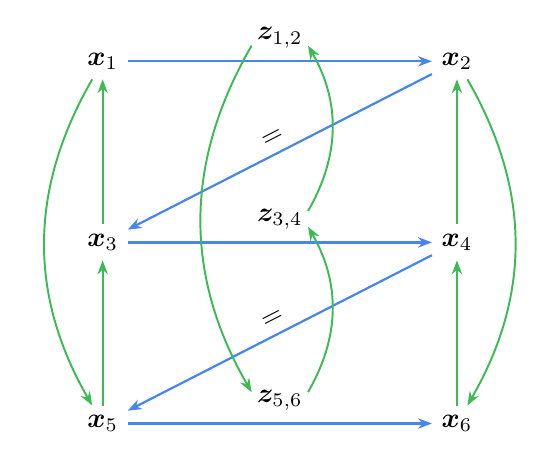
\begin{tikzpicture}
			\tikzset{
				zij/.style = {inner sep=0pt, outer sep=2pt, midway, above=0.1cm},
				comp/.style = {{Stealth[length=5pt]}-, draw=Gblue, thick}
			}
			\def\hgap{4.5}
			\def\vgap{2.3}
			\node (x1) at (0,0) {$\vecx_1$};
			\node (x2) at (\hgap, 0) {$\vecx_2$} edge[comp] node[zij] (z12) {$\vecz_{1,2}$} (x1);
			\node (x3) at (0,-\vgap) {$\vecx_3$} edge[comp] node[midway, sloped, above] (eq23) {$=$} (x2);
			\node (x4) at (\hgap, -\vgap) {$\vecx_4$} edge[comp] node[zij] (z34) {$\vecz_{3,4}$} (x3);
			\node (x5) at (0,-2*\vgap) {$\vecx_5$} edge[comp] node[midway, sloped, above] (eq45) {$=$} (x4);
			\node (x6) at (\hgap, -2*\vgap) {$\vecx_6$} edge[comp] node[zij] (z56) {$\vecz_{5,6}$} (x5);

			\path[-{Stealth[length=5pt]},line width=0.7pt,Ggreen]
			(x3) edge (x1)
			(x5) edge (x3)
			(x1) edge[out=-120,in=120] (x5)
			(x4) edge (x2)
			(x6) edge (x4)
			(x2) edge[out=-60,in=60] (x6)
			([shift={(0,0.1)}]z34.east) edge[out=60,in=-60] ([shift={(0,-0.1)}]z12.east)
			([shift={(0,0.1)}]z56.east) edge[out=60,in=-60] ([shift={(0,-0.1)}]z34.east)
			([shift={(0,-0.1)}]z12.west) edge[out=-120,in=120] ([shift={(0,0.1)}]z56.west);
		\end{tikzpicture}
		\end{center}

          \begin{claim}
            \label{cl:sigmaActsFreelyAndOrderp}
            The group $\a{\sigma}$ has order $p$ and acts freely on
            $\calV_{\vecg} \cap \overline{\calV_{\vech}}$.
          \end{claim}

          \begin{proof}              In order to see that $\abs{\sigma} = p$, note that the input of $\sigma$ consists
              of $3p$ blocks of variables. The permutation $\sigma$ performs a rotation of the
              first $2p$ blocks by two positions and of the last $p$ blocks by one
              position.
              All that remains is to show that $\a{\sigma}$ acts freely on
                    $\calV_{\vecg} \cap \overline{\calV_{\vech}}$.
                    First, we show that $\a{\sigma}$ defines a group action on
                    $\calV_{\vecg} \cap \overline{\calV_{\vech}} $, that is
                    for all $\vecx \in \calV_{\vecg} \cap
                    \overline{\calV_{\vech}}$, it holds that $\sigma(\vecx) \in
                    \calV_{\vecg} \cap \overline{\calV_{\vech}}$.
                    Let $\vecx = (\vecx_1, \vecx_2,
                    \dots, \vecx_{2p-1}, \vecx_{2p}, \vecz_{1,2}, \vecz_{3,4}, \dots, \vecz_{2p-
                    1,2p} ) \in \calV_{\vecg} \cap \overline{\calV_{\vech}} $,
                    then
                    \begin{itemize}
                        \item $\vecx \in \calV_{\vecg}$ implies that
                        $\vecf_{\calC}(\vecx_{2i-1},\vecx_{2i},
                        \vecz_{2i-1,2i}) = 0$ for $i \in \bracks{p}$ and
                        $\vecx_{2i} = \vecx_{2i+1}$ for $i \in \bracks{p-1}$
                        \item $\vecx \in \overline{\calV_{\vech}}$ implies that
                        $\vecx_1 \neq \vecx_2$, that is,
                        $\calC(\vecx_{1}) \neq \vecx_1$ since
                        $\vecf_{\calC}(\vecx_{1},\vecx_{2},
                        \vecz_{1,2}) = 0 \Leftrightarrow \vecx_2 =
                        \calC(\vecx_{1}) $.
                    \end{itemize}
                Now, $\sigma(\vecx) = (\vecx_{3}, \vecx_{4},
                \ldots, \vecx_{1}, \vecx_{2}, \vecz_{3,4}, \vecz_{5,6}, \ldots,
                \vecz_{1,2}) \in  \calV_{\vecg} \cap
                \overline{\calV_{\vech}}$ holds because
                \begin{itemize}
                    \item $\vecf_{\calC}(\vecx_{2i-1},\vecx_{2i},
                    \vecz_{2i-1,2i}) = 0$ for $i \in \bracks{p}$ and
                    $\vecx_{2i} = \vecx_{2i+1}$ for $i \in \bracks{p-1}$, which holds
                    from $\vecx \in \calV_{\vecg}$. Additionally, $\vecx_1 = \vecx_{2p}$ holds because we pre-processed $\calC$ such that $\calC^p(\vecx_1) = \vecx_{1}$,
                    \item $\vecx_{3} \neq \vecx_{4}$, which holds because
                    $\vecx_{4}  = \calC(\vecx_{3})$ for $i \in \bracks{p}$
                    and from the definition of $\calC$, $\calC(\vecx_{1})
                    \neq \vecx_1$ implies that $\vecx_{2i} \neq \vecx_{2i-1}$ for all
                    $i \in \bracks{p}$.
                \end{itemize}

              Finally, if $\vecx \in \calV_{\vecg} \cap
              \overline{\calV_{\vech}}$, by
              construction of $\cal{C}$, we have that $\vecx_{2k} \neq \vecx_{2j}$ for
              $k\neq j$ and thus $\sigma(\vecx) \ne \vecx$ simply because $\vecx_3 \ne \vecx_1$. Thus, we conclude that $\a{\sigma}$ acts freely on
              $\calV_{\vecg} \cap \overline{\calV_{\vech}}$.
          \end{proof}

        		\paragraph{Putting it all together.} The solution of this instance of $\cChevalleyp$ cannot be a vector
                $\vecx \in \calV_{\vecg} \cap \overline{\calV_{\vech}}$  with
                $\sigma(\vecx)
                \not\in \calV_{\vecg} \cap \overline{\calV_{\vech}}$ or
                $\sigma(\vecx) = \vecx$, since we know from
                \autoref{cl:sigmaActsFreelyAndOrderp} that $\a{\sigma}$ acts freely on
                $\calV_{\vecg} \cap \overline{\calV_{\vech}}$.
                We also have from \autoref{thm:labeledChevalleyWarningTheorem} that the solution also cannot be a max-degree monomial in the expansion of $\CW_{\vecg}(\bx) = \prod (1-g_i^{p-1})$.
                Thus, the solution must be an $\vecx \neq \vec{0}$ such that
                $\vecf(\vecx) = \vec{0}$. Let $\vecx_1$ denote the first $n$
                coordinates of $\vecx$, then $\vecf(\vecx) = \vec{0}$ implies that
                $\vecx_1 = \calC(\vecx_1)$ and $\vecx \neq \vec{0}$ implies that
                $\vecx_1 \neq \vec{0}$. Hence, $\vecx_1$ corresponds to
                a lonely vertex of the $\lonelyp$ instance.
\end{proof} 

\section*{Required restricted-Lonely support}
\setcounter{theorem}{43}
\begin{lemma}\label{lem:restricted-lonely}
	For all primes $p$ and $k \in \set{1, \ldots, p-1}$, $\lonely_p$ reduces to $\lonely_p^k$.
\end{lemma}

\appendix
\setcounter{section}{0}
\setcounter{theorem}{46}
\section{Appendix: Reductions Between Complete Problems}
\label{sec:equivalences}

In order to prove \autoref{thm:PPAqEquivalentProblems}, we introduce an additional problem that will serve as intermediate problem in our reductions.\\[1mm]


\noindent
\begin{minipage}{\linewidth}
\begin{definition}
	\label{def:leaf-prime} \contour{black}{($\leaf'_q$)}\vspace{-5pt}
	\begin{itemize}[leftmargin=2.15cm,itemsep=4pt]
		\item[\slshape Principle:] Same as $\leaf_q$, but degrees are allowed to be larger (polynomially bounded).
		\item[\slshape Object:] $q$-uniform hypergraph $G = (V, E)$. Designated vertex $v^* \in V$.
		\item[\slshape Inputs:] $\triangleright$ $C:\bit^n \to (\bit^{nq})^k$, with $(\bit^{nq})^k$ interpreted as $k$ many $q$-subsets of $\bit^n$\\
	$\triangleright$ $v^* \in \bit^n$ (usually $0^n$)
		\item[\slshape Encoding:] $V\coloneqq\bit^n$.\\
	For distinct $v_1, \ldots, v_q$, edge $e\coloneqq\set{v_1, \ldots, v_q}\in E$ if $e \in C(v)$ for all $v \in e$
		\item[\slshape Solutions:] $v^*$ if $\deg(v) \equiv 0 \mod{q}$ and\\
	$v \ne v^*$ if $\deg(v) \not\equiv 0 \mod{q}$
	\end{itemize}
\end{definition}
\end{minipage}\vspace{5mm}


\begin{proof}[Proof of \autoref{thm:PPAqEquivalentProblems}]
We show the following inter-reducibilities: (1) $\leaf_q \asymp \leaf_q'$, (2) $\leaf_q' \asymp \bipartite_q$ and (3) $\leaf_q \asymp \lonely_q$.

\medskip

\parasc{(1a) $\boldsymbol{\leaf_q \reducible \leaf_q'}$} Each instance of $\leafq$ is trivially an instance of $\leaf'_q$.

\medskip

\parasc{(1b) $\boldsymbol{\leaf'_q \reducible \leafq}$.} We start with a $\leaf'_q$ instance $(C, v^*)$, where $C$ encode a $q$-uniform hypergraph $G = (V, E)$ with degree at most $k$. Let $t = \ceil{k/q}$. We construct a $\leaf_q$ instance encoding a hypergraph $\overline{G} = (\overline{V}, \overline{E})$ on vertex set $\overline{V}\coloneqq V \times [t]$, intuitively making $t$ copies of each vertex.

In order to locally compute hyperedges, we first fix a canonical algorithm that for any vertex $v$ and any edge $e \in E$ incident on $v$, assigns it a label $\ell_v(e) \in [t]$, with at most $q$ edges mapping to the same label --- e.g. sort all edges incident on $v$ in lexicographic order and bucket them sequentially in at most $t$ groups of at most $q$ each. Note that we can ensure that for any vertex $v$ at most one label gets mapped to by a non-zero, non-$q$ number of edges. Moreover, if $\deg(v) \equiv 0 \mod{q}$, then exactly $q$ or $0$ edges are assigned to any label.

We'll assume that $\deg(v^*) \not\equiv 0 \mod{q}$, as otherwise, a reduction wouldn't be necessary. We let $(v^*, \ell^*)$ be the designated vertex of the $\leaf_q$ instance, where $\ell^*$ is the unique label that gets mapped to by a non-zero, non-$q$ number of edges incident on $v^*$.

For any vertex $(v, i) \in \overline{V}$, we assign it at most $q$ edges as follows: For each edge $e = \set{v_1, \ldots, v_q}$ such that $\ell_v(e)=i$, the corresponding hyperedge of $(v,i)$ is ${(v_1, \ell_{v_1}(e)), \ldots, (v_q, \ell_{v_q}(e))}$. It is easy to see that the designated vertex $(v^*, \ell^*)$ indeed has non-zero, non-$q$ degree. Moreover, a vertex $\deg(v,i) \notin \set{0, q}$ in $\overline{G}$ only if $v$ has a non-multiple-of-$q$ degree in $G$. Thus, solutions to the $\leaf_q$ instance naturally maps to solutions to the original $\leaf_q'$ instance.

By \autoref{rem:simplifications}, this completes the reduction since the edges are locally computable with black-box access to $C$ and $\overline{V}$ is efficiently indexable.

\medskip

\parasc{(2a) $\boldsymbol{\leaf'_q \reducible \bipartiteq}$.}
We start with a $\leaf'_q$ instance $(C, v^*)$, where $C$ encode a $q$-uniform hypergraph $G = (V, E)$. We construct a $\bipartite_q$ instance encoding a graph $\overline{G} = (\overline{V} \cup \overline{U}, \overline{E})$ such that $\overline{V} = V$ and $\overline{U} = \binom{V}{q}$, i.e. all $q$-sized subsets of $V$. We include the edge $(v,e) \in \overline{E}$ if $e \in E$ is incident on $v$. The designated vertex for the $\bipartite_q$ instance is $v^*$ in $\overline{V}$.

Clearly, all vertices $e \in \overline{U}$ have degree either $q$ or $0$. For any $v \in \overline{V}$, the degree of $v$ in $\overline{G}$ is same as its degree in $G$. Thus, any solution to the $\bipartite_q$ instance immediately gives a solution to the original $\leaf'_q$ instance. By \autoref{rem:simplifications}, this completes the reduction since the edges are locally computable with black-box access to $C$ and $\overline{V}$ and $\overline{U}$ are efficiently indexable (cf. \cite[\S2.3]{r31} for efficiently indexing $\overline{U}$).

\medskip

\parasc{(2b) $\boldsymbol{\bipartiteq \reducible \leaf'_q}$.} We start with a $\bipartite_q$ instance $(C, v^*)$ encoding a bipartite graph $\calG = (V \cup U,E)$ with maximum degree of any vertex being at most $k$. We construct a $\leaf'_q$ instance encoding a hypergraph $\overline{G} = (\overline{V}, \overline{E})$ such that $\overline{V} = V$ with designated vertex $v^*$.

First, we fix a canonical algorithm that for any vertex $u \in U$ with $\deg_{G}(u) \equiv 0 \mod{q}$ produces a partition of it's neighbors with $q$ vertices of $V$ in each part. Now, the set of $q$-uniform hyperedges incident on any vertex $v \in \overline{V}$ in $\overline{E}$ can be obtained as: for all neighbors $u$ of $v$, with $\deg_G(u) \equiv 0 \mod{q}$, we include a hyperedge consisting of all vertices in the same partition as $v$ among the neighbors of $u$ (we ignore neighbors $u$ with $\deg(u) \not\equiv 0 \mod{q}$).

Observe that $\deg_{\overline{G}}(v) \le \deg_{G}(v)$ and equality holds if and only if all neighbors of $v$ in $G$ have degree $\equiv 0 \mod{q}$. Hence for any $v \in \overline{V}$, if $\deg_{\overline{G}}(v) \ne \deg_G(v) \mod{q}$, then there exists a neighbor $u \in U$ of $v$ in $G$ such that $\deg(u) \not\equiv 0 \mod{q}$. Thus, if $v = v^*$ and $\deg_{\overline{G}}(v^*) \equiv 0 \mod{q}$, then either $\deg_G(v) \equiv 0 \mod{q}$ or we can find a neighbor $u$ of $v$ in $G$ with $\deg(u) \not\equiv 0 \mod{q}$. Similarly if for some $v \ne v^*$, we have $\deg_{\overline{G}}(v^*) \not\equiv 0 \mod{q}$, then either $\deg_G(v) \not\equiv 0 \mod{q}$ or we can find a neighbor $u$ of $v$ in $G$ with $\deg(u) \not\equiv 0 \mod{q}$. Thus, any solution to the $\leaf'_q$ instance gives us a solution to the original $\bipartite_q$ instance. This completes the reduction since $\overline{V} = \bit^n$ and the edges are locally computable with black-box access to $C$.

\medskip

\parasc{(3a) $\boldsymbol{\leaf_q \reducible \lonely_q}$.} We start with a $\leaf_q$ instance $(C, v^*)$, where $C$ encode a $q$-uniform hypergraph $G = (V, E)$ with degree at most $q$. If $\deg_G(v^*) = q$ or $0$, then we don't need any further reduction. Else, we construct a $\lonely_q$ instance encoding a $q$-dimensional matching $\overline{G} = (\overline{V}, \overline{E})$ on vertex set $\overline{V} = V \times [q]$. The designated vertices will be $V^* = \set{(v,q-i) : 1 \le i \le q - \deg(v^*)}$. Note that, $|V^*| = q - \deg_G(v^*)$ and hence $1 \le |V^*| \le q-1$.

In order to locally compute hyperedges, we first fix a canonical algorithm that for any vertex $v$ and any edge $e \in E$ incident on $v$, assigns it a unique label $\ell_v(e) \in [q]$ --- e.g. sort all edges incident on $v$ in lexicographic order and label them sequentially in $[q]$. In fact, we can ensure that an edge incident on $v$ get labeled within $\set{1, \ldots, \deg_G(v)}$.

For any vertex $(v, i) \in \overline{V}$, we assign it at most one hyperedge as follows:
\begin{itemize}[label=$\triangleright$]
\item If $\deg_G(v) = 0$, we include the hyperedge $\set{(v,i) : i \in [q]}$.
\item Else if $\deg_G(v) \ge i$, then for edge $e = \set{v_1, \ldots, v_q}$ incident on $v$ such that $\ell_v(e)=i$, the corresponding hyperedge of $(v,i)$ is ${(v_1, \ell_{v_1}(e)), \ldots, (v_q, \ell_{v_q}(e))}$.
\item Else if $0 < \deg_G(v) < i$, we leave it isolated.
\end{itemize}

It is easy to see that our definition of hyperedges is consistent and that the designated vertices $V^*$ are indeed isolated. Moreover, a vertex $(v,i)$ is isolated in $\overline{G}$ only if $1 \le \deg_G(v)\le q-1$. Thus, solutions to the $\leaf_q$ instance naturally maps to solutions to the original $\leaf_q'$ instance.

By \autoref{rem:simplifications}, this completes the reduction since the edges are locally computable with black-box access to $C$ and $\overline{V}$ is efficiently indexable.

\medskip

\parasc{(3b) $\boldsymbol{\lonely_q \reducible \leaf_q}$.} We start with a $\lonely_q$ instance $(C, V^*)$, where $C$ encode a $q$-dimensional matching $G = (V, E)$. We construct a $\leaf_q$ instance encoding a $q$-uniform hypergraph $\overline{G} = (\overline{V}, \overline{E})$ on vertex set $\overline{V}$ that will be specified shortly. We describe the hyperedges in $\overline{G}$ and it'll be clear how to compute the hyperedges for any vertex locally with just black-box access to $C$.

We start with $\overline{V} = V$. Our goal is to transform all vertices of degree $1$ to degree $q$, while ensuring that vertices of degree $0$ are mapped to vertices of degree not a multiple of $q$. Towards this goal we let $\overline{E}$ to be set of edges in $E$ in addition to $q-1$ canonical $q$-dimensional matchings over $V$. For example, for a vertex $v \coloneqq (x_1, \ldots, x_n) \in V = [q]^n$, the corresponding edges in $\overline{E}$ include an edge in $E$ (if any) and edges of the type $e_i = \set{(x_1, \dots, x_{i-1}, j, x_{i+1}, \dots, x_n) : j \in [q]}$ for $i \in [q-1]$ (note, this requires us to assume $n \geq q-1$). Adding the $q-1$ matchings increases the degree of each vertex by $q-1$. Therefore, vertices with initial degree $1$ now have degree $q$ and vertices with initial degree $0$ now have degree $q-1$. However, a couple of issues remain in order to complete the reduction, which we handle next.

{\em Multiplicities.} An edge $e \in E$ might have gotten added twice, if it belonged to one of the canonical matchings. To avoid this issue altogether, instead of adding edges directly on $V$, we augment $\overline{V}$ to become $\overline{V} \coloneqq V \cup \inparen{\binom{V}{q} \times [q-1]}$, i.e. in addition to $V$, we have $q-1$ vertices for every potential hyperedge of $G$. For any edge $e\coloneqq\set{v_1, \ldots, v_q} \in E$, instead of adding it directly in $\overline{G}$, we add hyperedge $\set{v, (e,1), (e,2), \ldots, (e,q-1)}$ for each $v \in e$. Note that, all vertices $(e,i) \in \binom{V}{q} \times [q-1]$ have degree $q$ if $e \in E$ and degree $0$ if $e \notin E$, so they are non-solutions for the $\leaf_q$ instance. For vertices in $V$, we still have as before that vertices with initial degree $1$ now have degree $q$ and vertices with initial degree $0$ now have degree $q-1$.

{\em Designated vertex.} In a $\leaf_q$ instance, we need to specify a single designated vertex $v^* \in \overline{V}$. If the $\lonely_q$ instance had a single designated vertex then we would be done. However, in general it is not possible to assume this (for non-prime $q$). Nevertheless, we provide a way to get around this. We augment $\overline{V}$ with $t = (q-1)(q-k) + 1$ additional vertices to become $\overline{V} \coloneqq V \cup  \inparen{\binom{V}{q} \times [q-1]} \cup \set{w_{i,j} : i \in [q-k],\ j \in [q-1]} \cup \set{v^*}$, where $v^*$ will eventually be the single designated vertex for the $\leaf_q$ instance.

Let $V^* = \set{u_1, \ldots, u_k} \subseteq V$ be the set of designated vertices in the $\lonely_q$ instance (note $1 \le k < q$). So far, note that $\deg_{\overline{G}}(u_i) = q-1$. The only new hyperedges we add will be among $u_i$'s, $w_{i,j}$'s and $v^*$, in such a way that $\deg_{\overline{G}}(u_i)$ will become $q$, the degree of all $w_{i,j}$'s will also be $q$ and degree of $v^*$ will be $q-k$.
\begin{itemize}[label=$\triangleright$, itemsep=3pt]
\item For each $u \in V^*$, include $\set{u, w_{1,1}, \ldots, w_{1,q-1}}$. So far, $\deg_{\overline{G}}(u) = q$ and $\deg_{\overline{G}}(w_{1,j}) = k$.
\item For each $j \in [q-1]$ and each $i \in \set{2, \ldots, q-k}$, include $\set{w_{1,j}, w_{i,1}, \ldots, w_{i,q-1}}$.\\
So far, $\deg_{\overline{G}}(w_{i,j}) = q-1$ for all $(i,j) \in [q-k] \times [q-1]$.
\item Finally, for each $(i,j) \in [q-k] \times [q-1]$, include $\set{v^*, w_{i,1}, \ldots, w_{i,q-1}}$.\\
Now, $\deg_{\overline{G}}(w_{i,j}) = q$ for all $(i,j) \in [q-k] \times [q-1]$ and $\deg_{\overline{G}}(v^*) = q-k$.
\end{itemize}

Thus, we have finally reduced to a $\leaf_q$ instance encoding the graph $\overline{G} = (\overline{V}, \overline{E})$ with $\overline{V} \coloneqq V \cup  \inparen{\binom{V}{q} \times [q-1]} \cup \set{w_{i,j} : i \in [q-k],\ j \in [q-1]} \cup \set{v^*}$. By \autoref{rem:simplifications}, this completes the reduction, since $\overline{V}$ is efficiently indexable (again, see \cite{r31} for a reference on indexing $\binom{V}{q}$) and the edges are locally computable using black-box access to $C$.
\end{proof}

\subsection{\boldmath Completeness of Succinct Bipartite}\label{sec:sucBipartite}


We introduce a new intermediate problem to show $\PPA_p$--completeness of $\sucBipartite_p$.\\[1mm]


\noindent
\begin{minipage}{\linewidth}
\begin{definition}
	\label{def:two-matchings} \contour{black}{($\twoMatchings_p$)}\vspace{-5pt}
	\begin{itemize}[leftmargin=2.15cm,itemsep=4pt]
		\item[\slshape Principle:] Two $p$-dimensional matchings over a common vertex set, with a vertex in exactly one of the matchings, has another such vertex.
		\item[\slshape Object:] Two $p$-dimensional matchings $G_0 = (V, E_0)$, $G_1 = (V, E_1)$. Designated vertex $v^* \in V$.
		\item[\slshape Inputs:] $\triangleright$ $C_0:\bit^n \to (\bit^n)^p$ and $C_1:\bit^n \to (\bit^n)^p$\\
	$\triangleright$ $v^* \in \bit^n$
		\item[\slshape Encoding:] $V\coloneqq\bit^n$. For $b \in \bit$, $E_b \coloneqq \set{e : C_b(v) = e \text{ for all } v \in e}$	
		\item[\slshape Solutions:] $v^*$ if $\deg_{G_0}(v^*) \ne 1$ or $\deg_{G_1}(v^*) \ne 0$ and\\
	$v \ne v^*$ if $\deg_{G_0}(v^*) \ne \deg_{G_1}(v^*)$
	\end{itemize}
\end{definition}
\end{minipage}\vspace{5mm}


\noindent Observe that in the case of $p=2$, $\twoMatchings_p$ can be readily seen as equivalent to $\leaf_2$.

\begin{theorem}\label{thm:succ-bip-complete}
	For any prime $p$, $\sucBipartite_p$ and $\twoMatchings_p$ are $\PPA_p$--complete.
\end{theorem}
\begin{proof}
We show that $\bipartite_p \reducible \sucBipartite_p \reducible \twoMatchings_p \reducible \lonely_p$.\medskip

\parasc{$\boldsymbol{\bipartitep \reducible \sucBipartitep}$.} Since $p$ is a prime, we can assume that the designated vertex $v^{*}$ has degree $1 \mod{p}$ (similar to \autoref{lem:restricted-lonely}). Since the
number of neighbors in a $\bipartitep$ instance are polynomial, we can
check if an edge exists and canonically group them efficiently for all vertices
with degree being a multiple of $p$. The designated edge $e^{*}$ is the unique ungrouped edge incident on $v^*$. Thus, valid solution edges to $\sucBipartite_p$ must have at least one endpoint which is a solution to the original $\bipartite_p$ instance.\medskip

\parasc{$\boldsymbol{\sucBipartitep \reducible \twoMatchingsp}$.}
We reduce to a $\twoMatchings_p$ instance encoding two $p$-dimensional matchings $\overline{G}_0 = (\overline{V}, \overline{E}_0)$ and $\overline{G}_1 = (\overline{V}, \overline{E}_1)$, over the vertex set $\overline{V} = V \times U \times [p-1]$, that is, all possible edges producible in the $\sucBipartite_p$ instance. The designated vertex $v^*$ is the designated edge $e^*$ in the $\sucBipartite_p$ instance.

For any edges $e_1, \ldots, e_p$, which are grouped by $\phi_V$ pivoted at some $v \in V$, we include the hyperedge $\set{e_1, \ldots, e_p}$ in $\overline{E}_0$. Similarly, for any edges $e_1, \ldots, e_p$, which are grouped by $\phi_U$ pivoted at some $u \in U$, we include the hyperedge $\set{e_1, \ldots, e_p}$ in $\overline{E}_1$. It is easy to see that points in exactly one of the two matchings $\overline{G}_0$ or $\overline{G}_1$ correspond to edges of the $\sucBipartite_p$ instance that are not grouped at exactly one end. Thus, we can derive a solution to $\sucBipartite_p$ from a solution to $\twoMatchings_p$. (Remark: while edges which are not grouped at either end are solutions to $\sucBipartite_p$, they do not correspond to a solution in the $\twoMatchings_p$ instance.) \medskip

\parasc{$\twoMatchings_p \reducible \lonely_p$.} Given a $\twoMatchings_p$ instance encoding two $p$-dimensional matchings $G_0 = (V, E_0)$ and $G_1 = (V, E_1)$, we reduce to an instance of $\lonely_p$ encoding a $p$-dimensional matching $\overline{G} = (\overline{V}, \overline{E})$ such that $\overline{V} = V \times [p]$. The designated vertex for the $\lonely_p$ instance is $(v^*,p)$.

For any hyperedge $\set{v_1, \ldots, v_p}$ in $E_0$, we include the hyperedge $\set{(v_1, i), (v_2, i), \ldots, (v_p,i)}$ in $\overline{G}$ for each $i \in \set{1, \ldots, p-1}$. Similarly, for any hyperedge $\set{v_1, \ldots, v_p}$ in $E_1$, we include the hyperedge $\set{(v_1, p), (v_2, p), \ldots, (v_p,p)}$ in $\overline{G}$. If $v \in V$ is isolated in both $G_0$ and $G_1$, then we include the hyperedge $\set{v} \times [p]$.

Observe that, $(v^*, p)$ is isolated by design. A vertex $(v,i)$, for $i < p$ is isolated only if $\deg_{G_0}(v) = 0$ and $\deg(G_1) = 1$. Similarly, the vertex $(v,p)$ is isolated only if $\deg_{G_0}(v) = 1$ and $\deg(G_1) = 0$. Thus, isolated vertices in the $\lonely_p$ instance correspond to solutions of the $\twoMatchings_p$ instance.
\end{proof}

\subsection{Restricted-Lonely support}\label{sec:pmod-equivalence}

\begin{proof}[Proof of \autoref{lem:restricted-lonely}]
Consider any prime $p$. Consider a $\lonely_p$ instance $(C, V^*)$, where $C$ encodes a $p$-dimensional matching $G = (V,E)$ and $|V^*| = \ell$. We wish to reduce to an instance of $\lonely_p^k$, where the number of designated vertices is exactly $k$. First, we'll assume that all vertices in $V^*$ are indeed isolated in $G$, otherwise, no reduction would be necessary. The key reason why this lemma holds for primes (and not for composites) is because $\ell$ has a multiplicative inverse modulo $p$. In particular, let $t \equiv \ell^{-1} k \mod{p}$.

We construct a $\lonely_p^k$ instance encoding the $p$-dimensional matching $\overline{G} = (\overline{V}, \overline{E})$ over $\overline{V} = V \times [t]$. We let $\overline{V}^*$ to be the lexicographically first $k$ vertices in $V^* \times [t]$. Note that $|V^* \times [t]| = t.\ell \equiv k \mod{p}$. Thus, we partition the remaining vertices of $V^* \times [t]$ into $p$-uniform hyperedges. For any vertex $v \in V \smallsetminus V^*$, with neighbors $v_1, \ldots, v_{p-1}$ in $G$, the neighbors of $(v,i)$ in $\overline{G}$ are $(v_1, i), \ldots, (v_{p-1}, i)$ for any $i \in [t]$. Thus, a vertex $(v,i)$ is isolated only if it is in $\overline{V}^*$ or $v$ is isolated in $G$. This completes the reduction since $\overline{V}$ is efficiently indexable -- see \autoref{rem:simplifications}.
\end{proof}



\begin{thebibliography}{37}
\bibitem{r1} James Aisenberg, Maria Luisa Bonet, and Sam Buss. 2-d tucker is PPA complete. Electronic Colloquium on Computational Complexity (ECCC), 22:163, 2015. URL: http://eccc.hpi-web. de/report/2015/163.
\bibitem{r2} Noga Alon. Splitting necklaces. Advances in Mathematics, 63(3):247–253, 1987. doi:10.1016/ 0001-8708(87)90055-7.
\bibitem{r3} Noga Alon, Shmuel Friedland, and Gil Kalai. Regular subgraphs of almost regular graphs. Journal of Combinatorial Theory, Series B, 37(1):79–91, 1984.
\bibitem{r4} Noga Alon and Douglas B. West. The Borsuk-Ulam theorem and bisection of necklaces. Proceedings of the American Mathematical Society, 98(4):623–628, 1986. doi: 10.1090/S0002-9939-1986-0861764-9.
\bibitem{r5} Paul Beame, Stephen A. Cook, Jeff Edmonds, Russell Impagliazzo, and Toniann Pitassi. The relative complexity of NP search problems. J. Comput. Syst. Sci., 57(1):3–19, 1998. doi:10.1006/jcss.1998.1575.
\bibitem{r6} Paul Beame and Søren Riis. More on the relative strength of counting principles. In Proceedings of the DIMACS Workshop on Proof Complexity and Feasible Arithmetics, volume 39, pages 13–35, 1998.
\bibitem{r7} Richard Beigel and John Gill. Counting classes: Thresholds, parity, mods, and fewness. Theor. Comput. Sci., 103(1):3–23, 1992. doi:10.1016/0304-3975(92)90084-S.
\bibitem{r8} Aleksandrs Belovs, Gábor Ivanyos, Youming Qiao, Miklos Santha, and Siyi Yang. On the polynomial parity argument complexity of the combinatorial nullstellensatz. In 32nd Computational Complexity Conference, CCC 2017, July 6-9, 2017, Riga, Latvia, pages 30:1– 30:24, 2017. doi:10.4230/LIPIcs.CCC.2017.30.
\bibitem{r9} Nir Bitansky, Omer Paneth, and Alon Rosen. On the cryptographic hardness of finding a nash equilibrium. In 2015 IEEE 56th Annual Symposium on Foundations of Computer Science, pages 1480–1498. IEEE, 2015.
\bibitem{r10} Josh Buresh-Oppenheim and Tsuyoshi Morioka. Relativized NP search problems and propositional proof systems. In 19th Annual IEEE Conference on Computational Complexity (CCC 2004), 21-24 June 2004, Amherst, MA, USA, pages 54–67, 2004. doi: 10.1109/CCC.2004.1313795.
\bibitem{r11} Joshua Buresh-Oppenheim. On the TFNP complexity of factoring. Manuscript, 2006. URL: http://www.cs.toronto.edu/~bureshop/factor.pdf.
\bibitem{r12} Samuel R. Buss, Dima Grigoriev, Russell Impagliazzo, and Toniann Pitassi. Linear gaps between degrees for the polynomial calculus modulo distinct primes. J. Comput. Syst. Sci., 62(2):267–289, 2001. doi:10.1006/jcss.2000.1726.
\bibitem{r13} Samuel R. Buss and Alan S. Johnson. Propositional proofs and reductions between NP search problems. Ann. Pure Appl. Logic, 163(9):1163–1182, 2012. doi:10.1016/j.apal.2012.01.015.
\bibitem{r14} I. Bárány, S. B. Shlosman, and A. Szücs. On a topological generalization of a theorem of tverberg. Journal of the London Mathematical Society, s2-23(1):158–164, 1981. doi: 10.1112/jlms/s2-23.1.158.
\bibitem{r15} Claude Chevalley. Démonstration d’une hypothèse de m. artin. Abhandlungen aus dem Mathematischen Seminar der Universität Hamburg, 11(1):73–75, December 1935. doi:10. 1007/BF02940714.
\bibitem{r16} Arka Rai Choudhuri, Pavel Hubácek, Chethan Kamath, Krzysztof Pietrzak, Alon Rosen, and Guy N Rothblum. Finding a nash equilibrium is no easier than breaking fiat-shamir. In Proceedings of the 51st Annual ACM SIGACT Symposium on Theory of Computing, pages 1103–1114. ACM, 2019.
\bibitem{r17} Constantinos Daskalakis, Paul W. Goldberg, and Christos H. Papadimitriou. The complexity of computing a nash equilibrium. SIAM J. Comput., 39(1):195–259, 2009. doi:10.1137/ 070699652.
\bibitem{r18} Constantinos Daskalakis and Christos H. Papadimitriou. Continuous local search. In Proceedings of the Twenty-Second Annual ACM-SIAM Symposium on Discrete Algorithms, SODA 2011, San Francisco, California, USA, January 23-25, 2011, pages 790–804, 2011. doi:10.1137/1.9781611973082.62.
\bibitem{r19} Xiaotie Deng, Jack R. Edmonds, Zhe Feng, Zhengyang Liu, Qi Qi, and Zeying Xu. Understanding PPA-Completeness. In Ran Raz, editor, 31st Conference on Computational Complexity (CCC 2016), volume 50 of Leibniz International Proceedings in Informatics (LIPIcs), pages 23:1–23:25, Dagstuhl, Germany, 2016. Schloss Dagstuhl–Leibniz-Zentrum fuer Informatik. doi:10.4230/LIPIcs.CCC.2016.23.
\bibitem{r20} Aris Filos-Ratsikas and Paul W. Goldberg. Consensus halving is ppa-complete. In Proceedings of the 50th Annual ACM SIGACT Symposium on Theory of Computing, STOC 2018, Los Angeles, CA, USA, June 25-29, 2018, pages 51–64, 2018. doi:10.1145/3188745.3188880.
\bibitem{r21} Aris Filos-Ratsikas and Paul W. Goldberg. The complexity of splitting necklaces and bisecting ham sandwiches. In STOC (to appear), 2019. arXiv:1805.12559.
\bibitem{r22} C. Goldberg and D. West. Bisection of circle colorings. SIAM Journal on Algebraic Discrete Methods, 6(1):93–106, 1985. doi:10.1137/0606010.
\bibitem{r23} Mika Göös, Pritish Kamath, Robert Robere, and Dmitry Sokolov. Adventures in monotone complexity and TFNP. In 10th Innovations in Theoretical Computer Science Conference, ITCS 2019, January 10-12, 2019, San Diego, California, USA, pages 38:1–38:19, 2019. doi:10.4230/LIPIcs.ITCS.2019.38.
\bibitem{r24} Michelangelo Grigni. A sperner lemma complete for ppa. Information Processing Letters, 77(5-6):255–259, 2001.
\bibitem{r25} Alexandros Hollender. The classes PPA-k: Existence from arguments modulo k. In Ioannis Caragiannis, Vahab Mirrokni, and Evdokia Nikolova, editors, Web and Internet Economics, pages 214–227, Cham, 2019. Springer International Publishing.
\bibitem{r26} Emil Jerábek. Integer factoring and modular square roots. J. Comput. Syst. Sci., 82(2):380–394, 2016. doi:10.1016/j.jcss.2015.08.001.
\bibitem{r27} Alan S. Johnson. Reductions and propositional proofs for total NP search problems. UC San Diego Electronic Theses and Dissertations, 2011. URL: https://escholarship.org/uc/ item/89r774x7.
\bibitem{r28} David S. Johnson, Christos H. Papadimitriou, and Mihalis Yannakakis. How easy is local search? J. Comput. Syst. Sci., 37(1):79–100, 1988. doi:10.1016/0022-0000(88)90046-3.
\bibitem{r29} Ilan Komargodski, Moni Naor, and Eylon Yogev. White-box vs. black-box complexity of search problems: Ramsey and graph property testing. Journal of the ACM (JACM), 66(5):34, 2019.
\bibitem{r30} Pravesh K Kothari and Ruta Mehta. Sum-of-squares meets nash: lower bounds for finding any equilibrium. In Proceedings of the 50th Annual ACM SIGACT Symposium on Theory of Computing, pages 1241–1248. ACM, 2018.
\bibitem{r31} Donald L. Kreher and Douglas R. Stinson. Combinatorial Algorithms: Generation, Enumeration, and Search, volume 7 of Discrete Mathematics and Its Applications. CRC Press, 1998.
\bibitem{r32} Nimrod Megiddo and Christos H. Papadimitriou. On total functions, existence theorems and computational complexity. Theor. Comput. Sci., 81(2):317–324, 1991. doi:10.1016/ 0304-3975(91)90200-L.
\bibitem{r33} Christos H. Papadimitriou. On the complexity of the parity argument and other inefficient proofs of existence. J. Comput. Syst. Sci., 48(3):498–532, 1994. doi:10.1016/S0022-0000(05) 80063-7.
\bibitem{r34} Christian Reiher. On kemnitz’conjecture concerning lattice-points in the plane. The Ramanujan Journal, 13(1-3):333–337, 2007.
\bibitem{r35} Aviad Rubinstein. Settling the complexity of computing approximate two-player nash equilibria. In IEEE 57th Annual Symposium on Foundations of Computer Science, FOCS 2016, 9-11 October 2016, Hyatt Regency, New Brunswick, New Jersey, USA, pages 258–265, 2016.
\bibitem{r36} Katerina Sotiraki, Manolis Zampetakis, and Giorgos Zirdelis. Ppp-completeness with connections to cryptography. In 59th IEEE Annual Symposium on Foundations of Computer Science, FOCS 2018, Paris, France, October 7-9, 2018, pages 148–158, 2018. doi: 10.1109/FOCS.2018.00023.
\bibitem{r37} Ewald Warning. Bemerkung zur vorstehenden arbeit von herrn chevalley. Abh. Math. Sem. Univ. Hamburg, 11:76–83, 1936.
\end{thebibliography}
\end{document}
